\section{Introduction}

In the previous chapter, we presented an initial modeling to reduce the carbon emissions of operating a cloud federation for the short term (one year) by sizing its renewable infrastructure, that is, defining the area of solar panels and capacity of the batteries for each data center.  Given that the cloud federation will operate for the long term, the decision-maker needs to be sure of the investments that will be made to avoid wasting money and as well generating more environmental impact with a bad strategy. Furthermore, a planing process is subject to many uncertainties that if not taken into account will decrease the validity and credibility of the solution.

This chapter will present an extension of the model focusing on the long-term operation of the cloud DCs and the uncertainties that this sizing process is subject to. In our context, the uncertainty comes mainly from the intermittency of renewables sources, therefore the reader will find in the next sections an analysis of the sensitivity of the modeling to the climate conditions.  Other input that may affect the sizing process is the value of the local electricity grid emissions. In our initial modeling we used the average value of the year, given that not all locations provide this value with shorter intervals --- hour by hour variation, for example. The reader will also find an analyisis of the impact of using the fine-grain information of the grid emissions in comparison of the average of the year on the sizing process and the resulting total carbon footprint.

Given that now the focus is in the long-term operation, it is essential to consider all the life cycle of the renewable infrastructure. On the previous chapter, we made the modeling considering only the environmental impact of manufacturing the solar panels and the lithium-ion batteries. This decision was made because it was the available data that we found at the time of studying the problem. However, the environmental impact also is present on the other phases of the life time of these devices --- as operation, discarding and recycling. Therefore, the modeling will be updated to account for the emissions of the life cycle of the renewable infrastructure. 

The reduction on the carbon emissions by using solar panels is limited by the fact that they only generates power when the sun is shinning, therefore they need to supply the operations of the cloud during the day and charge the batteries for night operations. In this chapter we will evaluate if using wind turbines could further reduce the carbon emissions of the cloud operation, and the sizing of both the PV panels and batteries --- considering that the wind may also be available at night.

One must also take into account that once built the renewable infrastructure cannot be reduced --- this would imply on destroying/discarding PV panels, batteries, and wind turbines. Therefore another strategy is necessary to deal with the over-sizing that might be caused by the intermittency of renewables sources. Thankfully, there is another part that can be managed to reduce the impact of bad-sizing: scheduling of the workload. In cloud platform, a significant part of the workload are tasks that does not have a high prioriry and whose execution can be delayed over time, the so-called batch tasks: at Meta, 7.5\% of the workload are offline tasks \cite{acun2022holistic} and low priority tasks consumes in average 20\% of the computational resources (CPU and memory) of Google's clusters \cite{googleborg_2020}. We will show an analysis of the vialbiliy of delaying $\alpha$ \% of the tasks up  to $\beta$ time slots (each time slot has 1 hour of duration) to reduce the carbon footprint.

Another important aspect to consider is that the demand for cloud computing resources grows year by year --- to deal with the increasing number of users and request of applications, and each year new servers generations are launched that have hardware more computational powerfull and that may be more energy efficient. As show by \citet{masanet2020recalibrating}, from 2010 to 2018 the DC workload increased 6 times, however the increase in energy consumption was only 6\% thanks to efficiency improvements in both hardware and software.  On the other hand, manufacturing these serves also emmits carbon and this cannot be neglected. Furthermore, given the increasing integration of renewable infrastructures in the cloud data centers, most of carbon emissions are shifting from the power consumption of the DC operation to the manufacturing of IT equipment \cite{gupta2021_chasingcarbon}.
Until now, we only explored the envonrimental impact aspect --- in terms of carbon emissions --- of the cloud federation operation. Another dimension of high importance for the decision maker is the monetary costs, since the business will only survive if it generates profit. The reader will find an analysis of how expensive is to reduce the carbon fooprint of the multi-cloud operation by using a local renewable infrastructure. Similar to the environmental impact analysis, we also take into account the costs of the whole life of the solar panels, wind turbines and batteries. 

More specifically, the chapter presents the following contributions:

\begin{itemize}
 
\item we extend the modeling to account for all the life cycle emissions of the renewable infrastructure --- from manufacturing to discarding/recycling
\item we present an evaluation of how much the carbon footprint could be reduced if wind turbines are also included inbthe renewable infrastructure 
\item we will show an evaluation regarding the sensitivity of the LP to the inputs: i) uncertainties caused by the intermittency of solar irradiation, and wind speed, and what needs to be considered in the modeling to avoid over or under-sizing of the renewable infrastructure; ii) some locations have data sources with grid carbon footprint at time intervals of one hour, and we will show an analysis if this fine-grain value would affect the renewable infrastructure sizing
\item we will how much we can reduce the carbon footprint using the flexibility of the schedulling --- delaying batch tasks
\item we will show an analysis of how expensive (in dollars) is to reduce the cloud federation footprint and the gains in both monetary and emissions savings
\item we will present an analysis of when is viable to add new servers (that may replace servers from older generations) in terms of carbon footprint


\end{itemize}

The remaining of the chapter is organized as follows. Considering that we are extending the model of the previous Chapter to evaluate different scenarios, each scenario will have its own Section --- Sections~\ref{sec:lifecicle}, ~\ref{sec:add_wt}, ~\ref{sec:sensitivity}, ~\ref{sec:flexibility}, ~\ref{sec:costs}, and  ~\ref{sec:new_servers}, and in each section the reader will find the necessary modifications in the modeling, the experiments performed and the results of the experiments. After presenting the evaluated scenarios, we will show the discussion at Section~\ref{sec:long_term_discussion}. Finally, Section~\ref{sec:long_term_conclusion} concludes the chapter.



\section{Life-cycle of the renewable infrastructure}
\label{sec:lifecicle}
\subsection{Updates in the model}

To model the carbon footprint taking into account the whole life cycle of the renewable infrastructure,  we will use the emissions of the energy produced (or
delivered in the case of batteries) in $g\,\ch{CO2}-eq.Wh^{-1}$ . Equation~\eqref{eq:fppv_lca} models the new footprint for the PV panels, and the main difference is the $pvCO2LC$ input that represents the life-cycle emissions.

\begin{equation} \label{eq:fppv_lca}
   FPpv^d_k =  pvCO2LC \times Pre_k^d \times \Delta t
\end{equation}


For the batteries, the initial modeling considered the emissions of manufacturing related to its capacity. Now to account for all the life-cycle, the emissions relate to the energy delivered (discharged) by the batteries. Equation~\eqref{eq:fbat_lca} models the new footprint for batteries, where $batCO2LC$ represents the life-cycle emissions. 

\begin{equation} \label{eq:fbat_lca}
   FPbat^d_k =  Pdch^d_k \times batCO2LC
 \end{equation}


Considering that now the information used for computing the  batteries emissions is the power discharged, we need to add a restriction for the batteries being used only for night computations, otherwise the solver will compute a solution where the batteries will be oversized to store all the excess of renewable energy during summer to supply during winter, resulting in GWh of capacity --- which is a problem considering the other environmental impact of batteries as their recycle rates needs yet to improve \cite{batteries_baumman}. Equation~\eqref{eq:b_initial_level}  models this resctriction, where $SUNRISE^d$ is the set with all the instants of times where the sun starts shining throghout the year in each location considering its time zone.

\begin{equation} \label{eq:b_initial_level}
  \forall t \in SUNRISE^d :  B^d_t =  0.2 \times Bat^d
\end{equation}

\subsection{Experiments}
\label{sec:ex_lca_pv}

\subsubsection{Settings} 

The cloud infrastructure, the workload, grid emissions, and the execution environment are the same as in Section  \ref{sec:settings_ccgrid}. For the photovoltaic power production, we will use the average of the irradiation from the years 1980 to 2019, and Figure \ref{fig:pv_ghi_avg} illustrates the values for the different DCs locations. This modification was to consider the variations between the years, as using a single year is not enough: it may be the case of a year with lowest or highest solar irradiation. More details for choosing the average irradiation value will be given in the next section.

\begin{figure}[h]  
  \centering
   {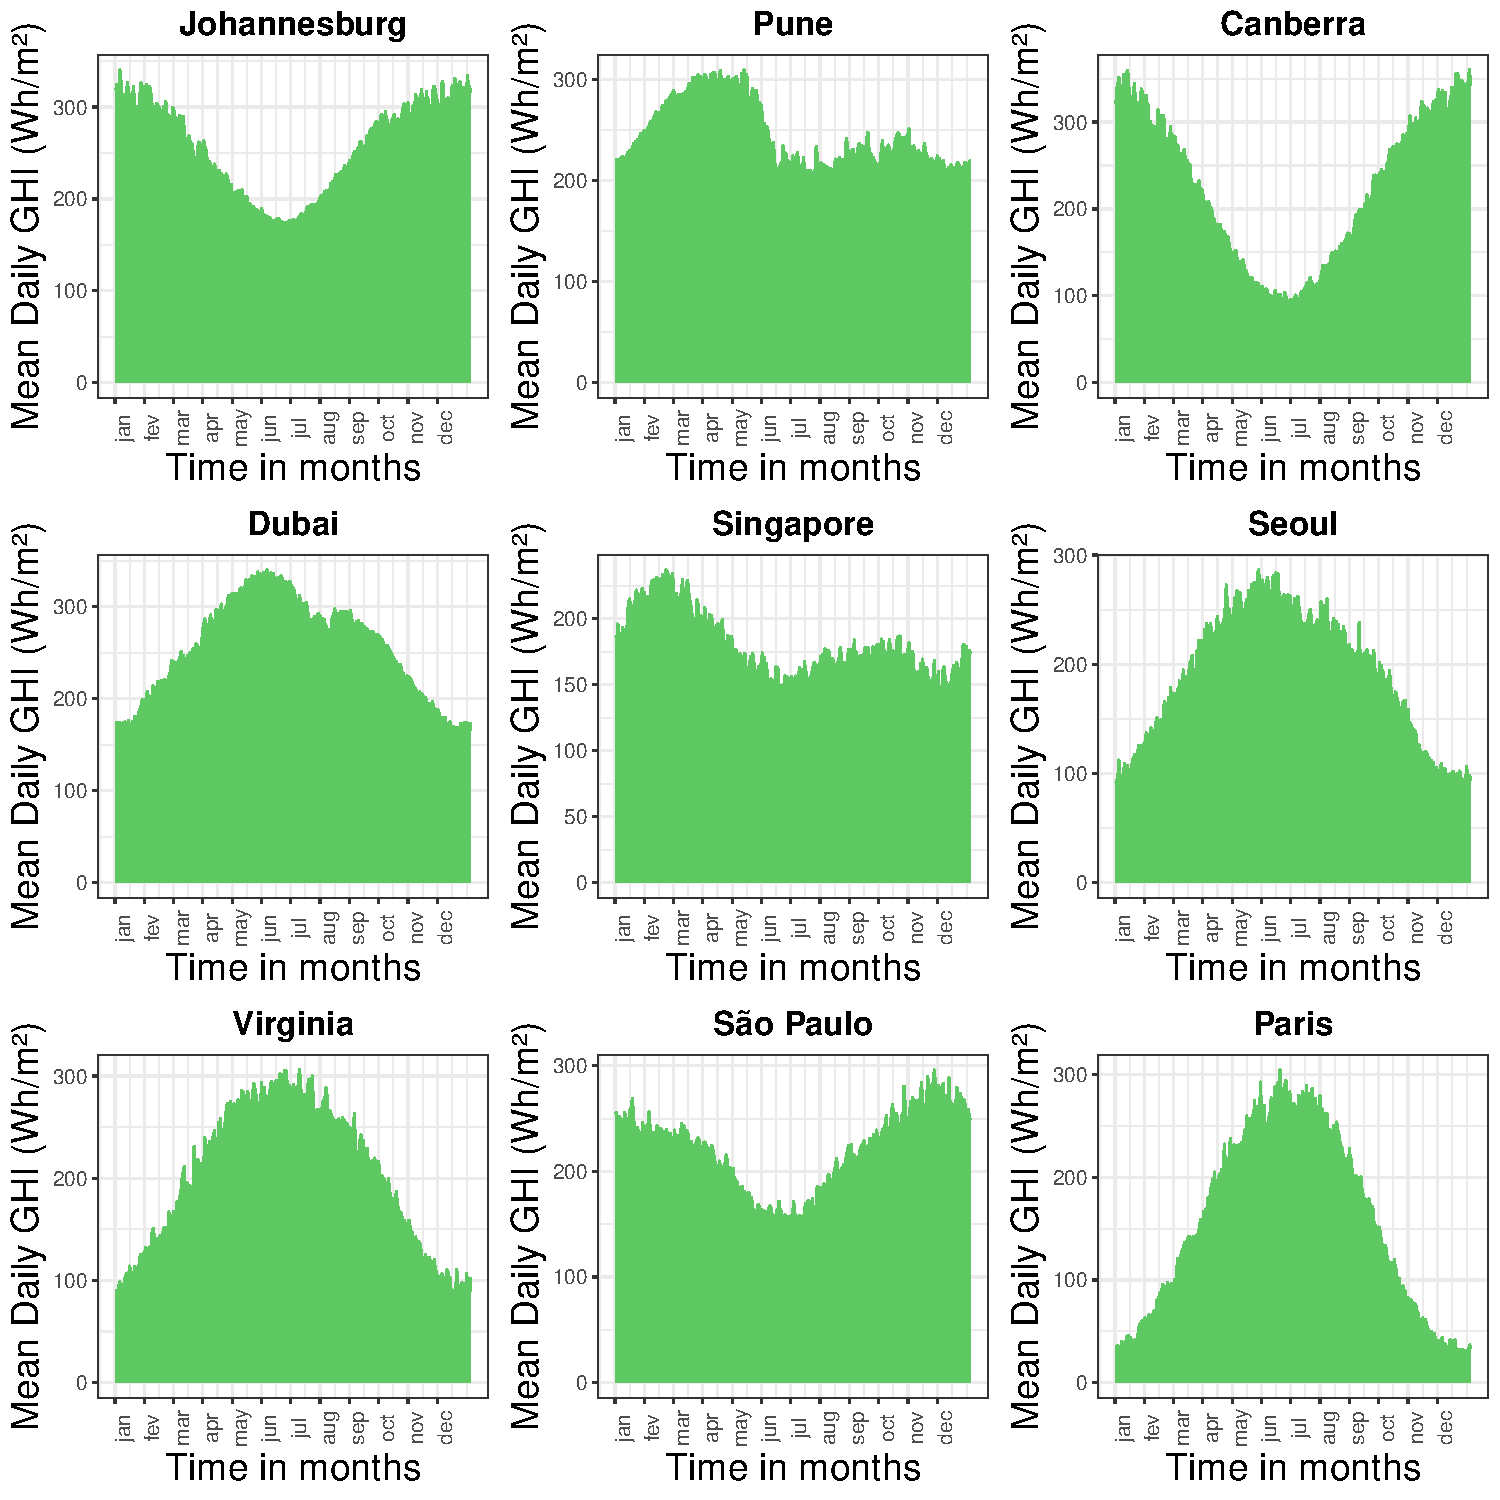
\epsfig{file = images/pv_daily_ghi_avg.pdf, width = .8\linewidth}}
   \caption{Average solar irradiation from 1980 to 2019 per location.}
  \label{fig:pv_ghi_avg}
\end{figure}

For the \ch{CO2} emissions of the batteries and PV whole life-cycle, we used values from the National Laboratory of Renewable Energy (NREL) of the United States that performed an analysis with over 3000 published studies on the life-cycle of renewable infrastructures \cite{nrel_lifecycle_2021}: $43 g\,\ch{CO2}-eq.Wh^{-1}$ for the PVs and $33 g\,\ch{CO2}-eq.Wh^{-1}$ for the Lithium-Ion batteries.

\subsubsection{Results}

Table~\ref{tab:emissions_LCA} presents the \ch{CO2} emissions of considering the whole life cycle in comparison with considering only the one from the manufacturing. As expected, the total \ch{CO2} emissions are higher (around 8\% of increase) since now the whole life cycle of the renewable infrastructure is taken into account. 

\begin{table}[!ht]
  
\caption{Total emissions for the different scenarios.}\label{tab:emissions_LCA} \centering

\begin{tabular}{|l|r|}
  \hline
  \textbf{Scenarios} & \textbf{Emissions ($t\,\ch{CO2}-eq$)}   \\
  \hline  
    \ch{CO2} from manufacturing   & 34559.03    \\  
  \hline
    \ch{CO2} from the whole life cycle       & 37828.49    \\
  \hline


\end{tabular}
\end{table}


Finally, in order to better assess the impact of considering the emissions from the whole life cycle in the sizing process, we compare its results with the sizing process that only considers the emissions from the manufacturing phase --- Figures~\ref{fig:pv_lca} and ~\ref{fig:bat_lca}.


% TODO add figures

\begin{figure}[h]
  \centering
  {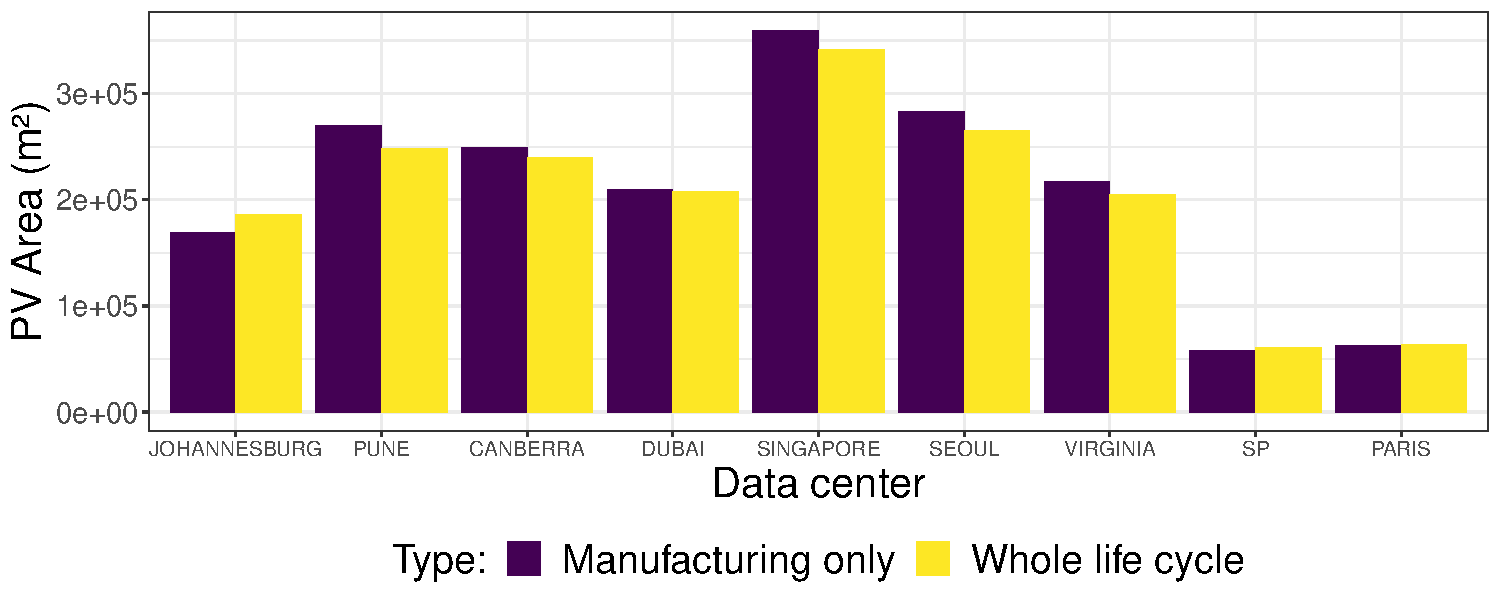
\epsfig{file = images/pv_sizing_after_lca.pdf, width = .8\textwidth}}
  \caption{PV Area sizing when considering carbon footprint of manufacturing vs whole life cycle. }
  \label{fig:pv_lca}
\end{figure}


\begin{figure}[h]
  \centering
  {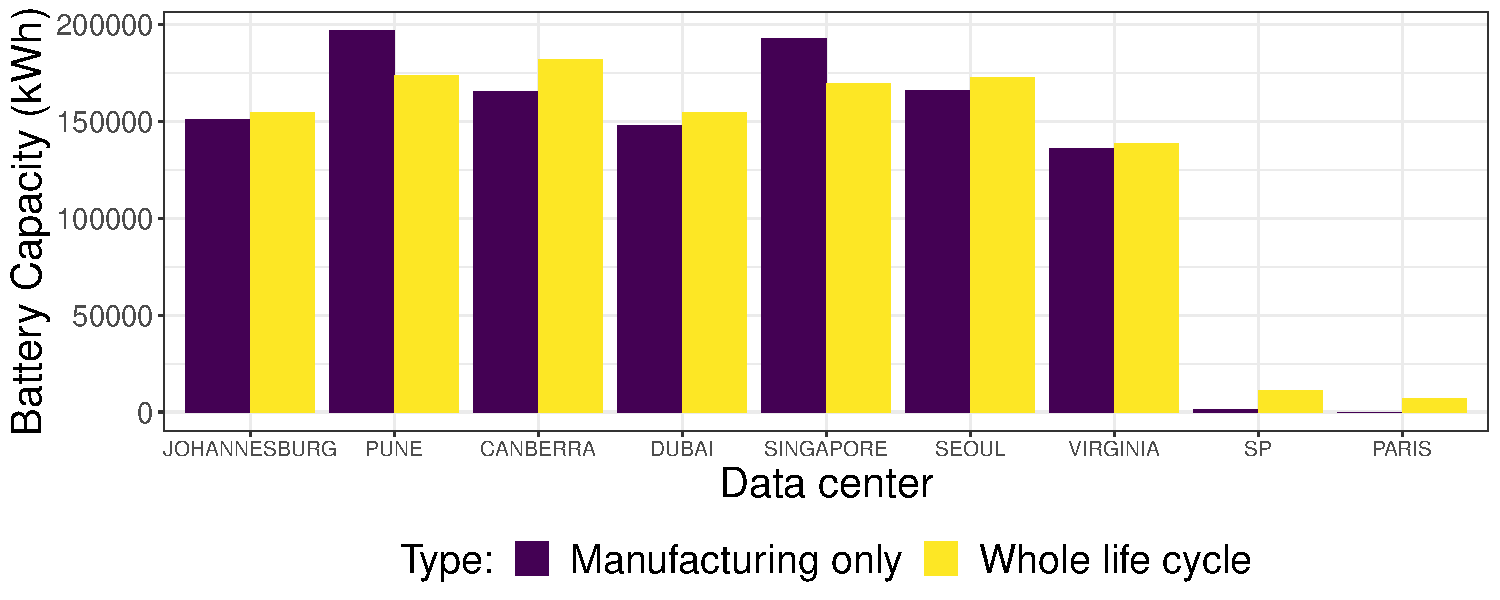
\epsfig{file = images/bat_sizing_after_lca.pdf, width = .8\textwidth}}
  \caption{Battery capacity sizing when considering carbon footprint of manufacturing vs whole life cycle.  }
  \label{fig:bat_lca}
\end{figure}



\section{Including wind turbines to the renewable infrastructure}
\label{sec:add_wt}
In this section, we will evaluate the impact adding other renewable power source: wind turbines, and to what extent they complement the photovoltaic power production to reduce the total emissions of the cloud federation operation, in particular during the night and seasons with lower solar irradiation as the winter.

\subsection{Updates in the model}
\label{sec:ex_model_wt}

We consider a new variable $WT^d$ that represents how much wind turbines will be built at each DC location. The number of wind turbines (WT) is an integer number (we cannot produce 1.2 WT for example). However, to avoid increasing the computational complexity of the LP by including integer variables, we made a relaxation in our modeling to allow the WT variable to be linear. 

The power production of the $WT^d$ wind turbines at location of data center $d$ at instant $k$ ($Pwt^d_{k}$) is modeled by Equation~\ref{eq:wt_power_prod}, where $V^d_k$ is the wind speed at location of data center $d$ at instant $k$; $Vici$ is the \textit{cut in} wind speed, that is, the wind turbines start producing power when the wind speed is greater or equal to $Vici$; $Vco$ is the \textit{cut out} wind speed, that is, the wind turbines stop producing power when the wind speed is greater than $Vco$; $Pr$ is the WT rated power production in W; and $Vr$ is the speed where the WT starts producing $Pr$ power. This model is based from \cite{HADDAD2021100505}.

\begin{equation} \label{eq:wt_power_prod}
Pwt^d_{k} = WT^d \times \left\{ 
  \begin{array}{ c l }
    0   & \quad \textrm{if } V^d_k \leq Vici \\
    Pr \times \frac{V^d_k - Vici}{Vr - Vici}  & \quad \textrm{if } Vici < V^d_k \leq Vr \\
    Pr  & \quad \textrm{if } Vr < V^d_k \leq Vco \\
    0  & \quad \textrm{if } Vco < V^d_k \\
  \end{array}
\right.
\end{equation}


Given that we are using an additional renewable power infrastructure, it is also necessary to update the model of the renewable power production on DC $d$ at instant $k$. Equation~\eqref{eq:new_renewable_power} models that the renewable power can be originated from both the PVs and WT.

\begin{equation} \label{eq:new_renewable_power}
    Pre^d_{k}= Ppv^d_{k} + Pwt^d_{k}
\end{equation}


To model the carbon footprint of the wind turbines, its whole life cycle also needs to be taken into account. Equation~\eqref{eq:fp_using_wt} models the footprint of using the WT at location of data center $d$ at instant $k$, where $wtCO2LC$ is the input that represents its emissions for the life cycle ( in $g\,\ch{CO2}-eq.Wh^{-1}$).

\begin{equation}\label{eq:fp_using_wt}
   FPwt^d_k =  wtCO2LC^d \times Pwt^d_{k}\times \Delta t
\end{equation}

Finally, the objective function also needs to be modified in order to include the carbon emissions of using WTs. Equation~\ref{eq:new_obj_co2} models the new objective function.

\begin{equation} \label{eq:new_obj_co2}
  \text{minimize }\sum_{k=0}^{K-1} \sum_{d=1}^D ( FPgrid^d_k +  FPpv^d_k +  FPwt^d_k + FPbat^d_k) 
\end{equation}

\subsection{Experiments}

\subsubsection{Settings}

The cloud infrastructure, the workload, grid emissions, and the execution environment are the same as in Section \ref{sec:settings_ccgrid}. The solar irradiation values, and emissions from PV panels and batteries are the same as Section \ref{sec:ex_lca_pv}. For the \ch{CO2} emissions of the wind turbines, it is considered that it emits $13 g\,\ch{CO2}-eq.Wh^{-1}$ taking into account its life cycle. The source for the values was the same as in Section \ref{sec:ex_lca_pv}, the analysis from NREL that evaluated more than 3000 studies.

For the wind speed data, we used values from the ERA5 data-source \cite{era5_wind_2022}. They provide values for the 100m v-component of wind (air horizontal speed towards the east) and 100m u-component of wind (air horizontal speed towards the north) --- both values are at 100 m of height. To transform these values into wind speed, we need to execute the following computation using the Pitagora's theorem: $ w_s = \sqrt{ v^2 + u^2} $, where $w_s$ is the wind speed, $u$ the value of the u-component and $v$ the value of the v-component.

\subsubsection{Results}

To evaluate the impact of including WT, we compare the sizing for using only PVs and batteries and using PV, batteries and WT. Table~\ref{tab:total_wind_and_pv_co2} presents the results in terms of total emissions when also considering the wind as renewable, we observe a reduction of approximately 34\% in comparison with the scenario where no WT is used and renewable energy is only produced by the PVs.

\begin{table}[h]  
  \caption{Total emissions (tons of \ch{CO2} for different scenarios }\label{tab:total_wind_and_pv_co2} \centering  
  \begin{tabular}{|l|r|}
  \hline    
  \textbf{Scenario} &   \textbf{Total \ch{CO2} emissions (tons)} \\
  \hline    
  PV + Bat + WT + Grid  & 24977.89 \\    
  \hline
  PV + Bat + Grid       & 37828.49 \\    
  \hline
\end{tabular}  
\end{table}


Table~\ref{tab:results_wt} presents the number of WTs manufactured at each data center location, as said in Section \label{sec:ex_model_wt}, we use a linear number for the wind turbines to avoid increasing the computational complexity of the problem. The decision-maker could decide whether rounding the value up or down based in its budget constraints.


\begin{table}[h]
  \caption{Computed number of WT for each location}\label{tab:results_wt} \centering
  \begin{tabular}{|l|r|}
  \hline
    
  \textbf{Location} &   \textbf{Number of WT} \\
  \hline
  Johannesburg & 58.11   \\
  \hline
  Pune  & 25.77 \\
  \hline
  Canberra  & 66.56 \\
  \hline
  Dubai   &  79.09  \\
  \hline
  Singapore & 36.93  \\
  \hline     
  Seoul    & 109.56  \\
  \hline
  Virginia   & 39.16 \\
  \hline
  São Paulo   & 86.53 \\
  \hline 
  Paris    &   22.15 \\
  \hline
  
\end{tabular}  
\end{table}



Finally, to assess the impact of including the WT regarding the sizing of both PV and batteries, we present in Figure~\ref{fig:wind_pv} and Figure~\ref{fig:wind_bat}  the dimensioning for both equipment considering and not considering manufacturing WT.  It is possible to observe that the inclusion of wind turbines has a significative reduction in the total solar panels area, and for some locations --- as São Paulo and Paris --- the optimal is to use only wind turbines. The batteries are also reduced, given that the wind can blow in the night as well, so no extra energy needs to be charged in the batteries from the solar panels to be used for night computations.



\begin{figure}[H]
  \centering
  {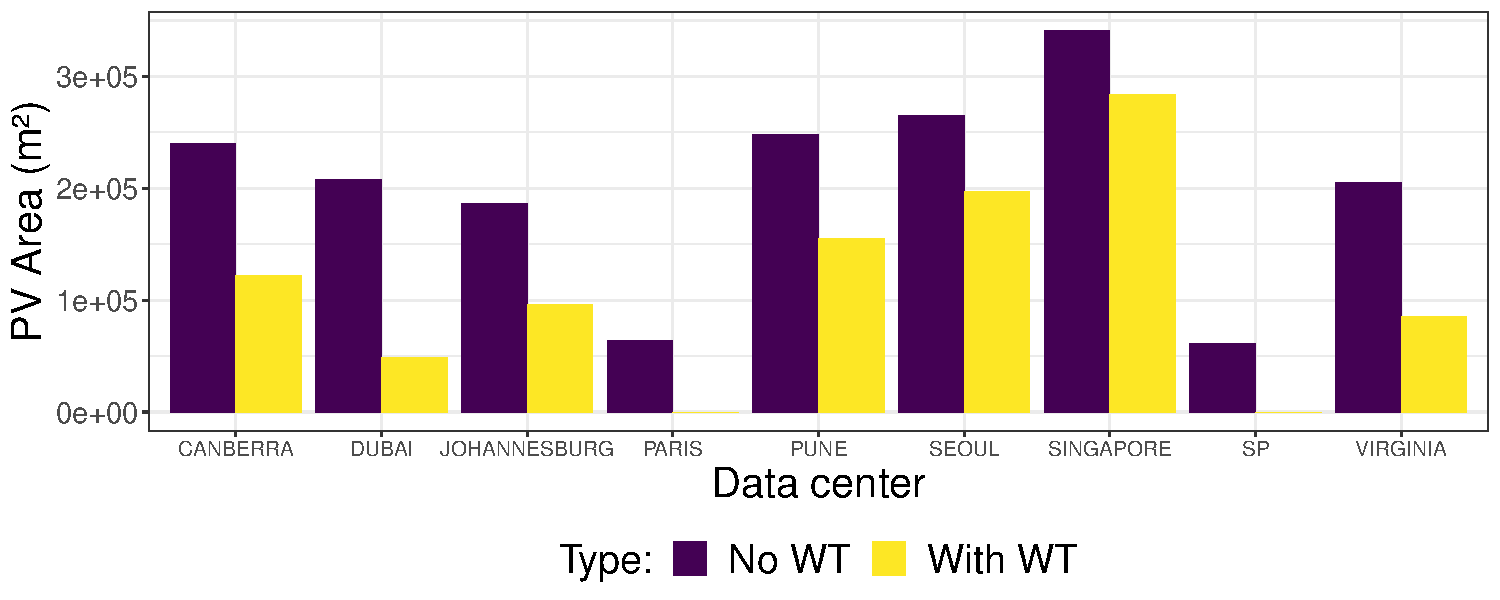
\epsfig{file = images/pv_sizing_after_wt.pdf, width = .8\textwidth}}
  \caption{PV Area sizing when the WT are and are not included }
  \label{fig:wind_pv}
\end{figure}


\begin{figure}[H]
  \centering
  {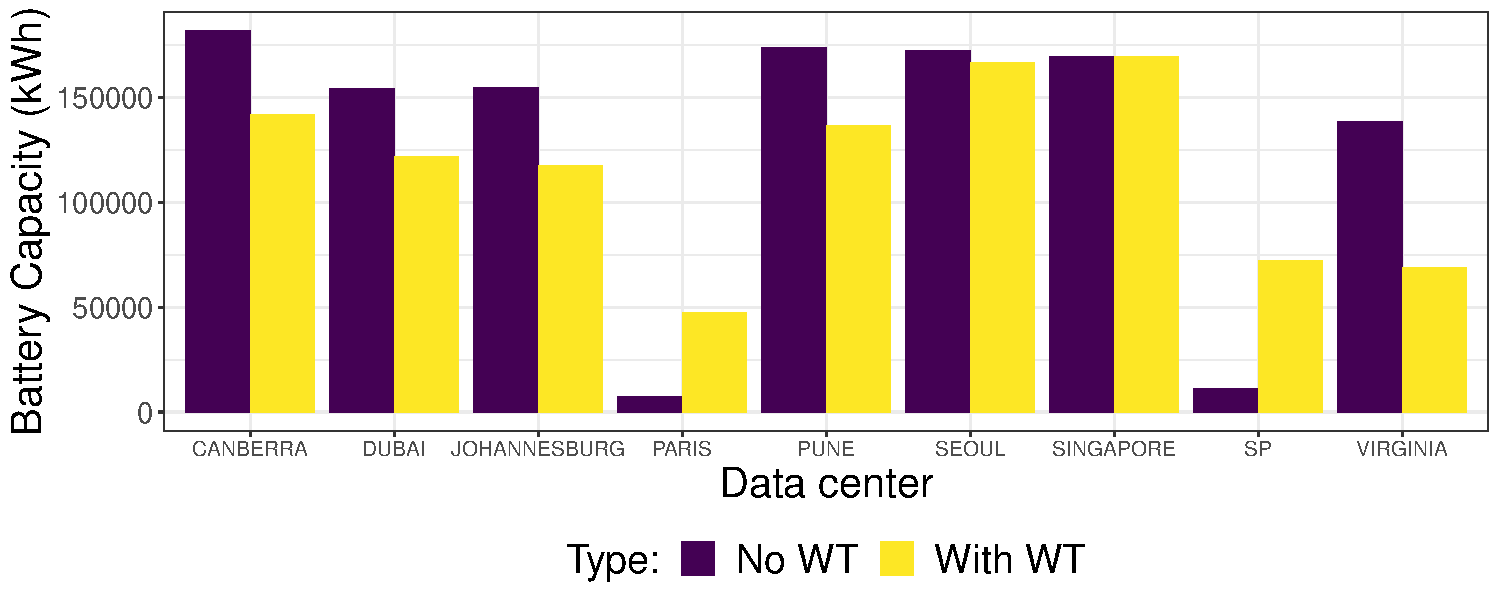
\epsfig{file = images/bat_sizing_after_wt.pdf, width = .8\textwidth}}
  \caption{Battery capacity sizing when the WT are and are not included }
  \label{fig:wind_bat}
\end{figure}


\section{Sensibility of the LP to  uncertainties}
\label{sec:sensitivity}
To assess the sensibility of the linear program to the inputs, we will evaluate it considering different scenarios in terms of solar irradiation, wind speed and grid emissions data. The renewables sources are intermittent by nature, and this variation can impact the sizing processing resulting in a over or under-sizing of the renewable infrastructure. To illustrate the intermittency of both wind speed and solar irradiation, we present in Figure~\ref{fig:pv_boxplots} boxplots of the total energy 1 solar panel produce per year during the years 1980 to 2019, and in Figure~\ref{fig:wt_boxplots} for a single wind turbine. Those figures ilustrates the intermittency of the renewable producton over the years, and one may also observe the potential for using one source or another: for example, Paris has the lowest solar power production considering 1 solar panel, and on the other hand, has the highest wind power production. 


\begin{figure}[h]
  \centering
  {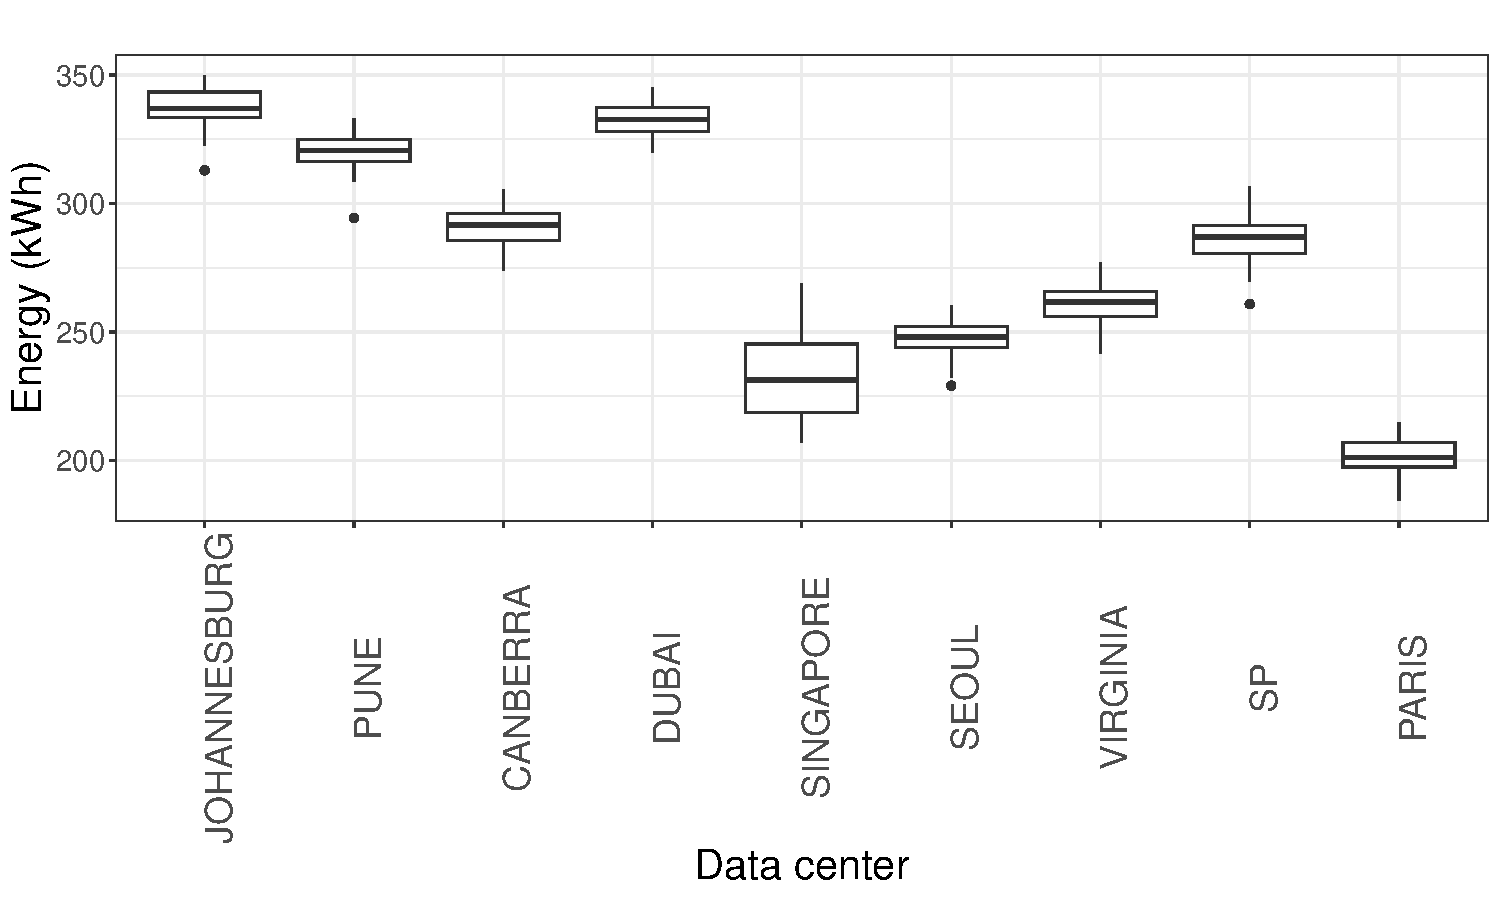
\epsfig{file = images/energy_pv.pdf, width = .8\textwidth}}
  \caption{Different energy production for 1 PV panel at each location for the years 1980 to 2019.}
  \label{fig:pv_boxplots}
\end{figure}


\begin{figure}[h]
  \centering
  {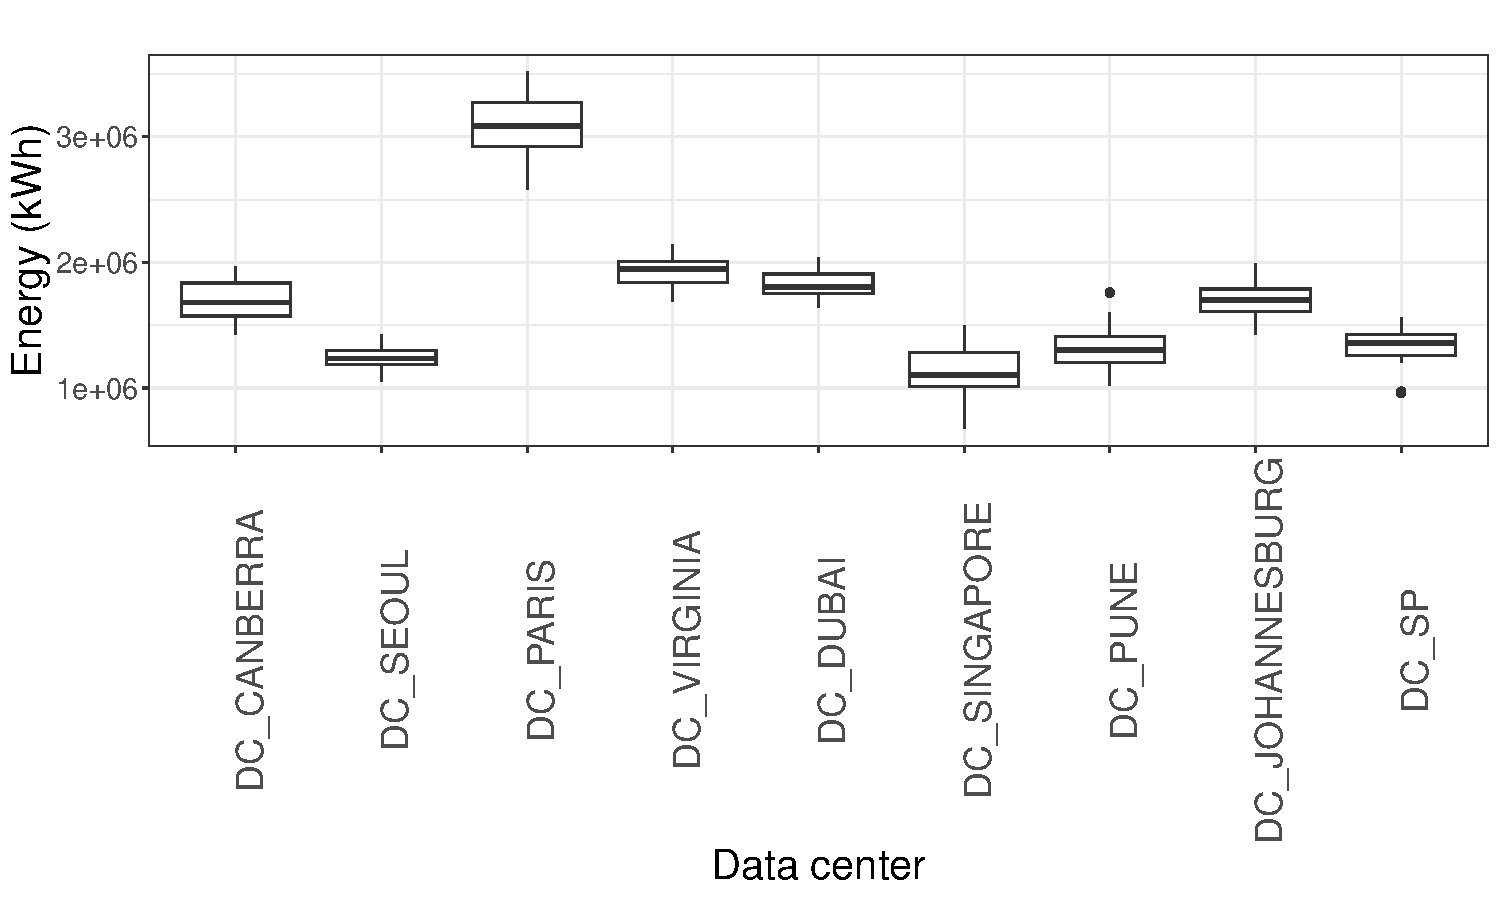
\epsfig{file = images/energy_wt.pdf, width = .8\textwidth}}
  \caption{Different energy production for 1 wind turbine at each location for the years 1980 to 2019.}
  \label{fig:wt_boxplots}
\end{figure}



Given the presence of low-carbon intensive sources in some countries, the emissions of the local electricity grid is not static all over the year, for example, regions that have access to solar energy have a lower grid footprint during the day. Some countries provide access to fine-grain information of its electricity mix in real time or historical data in the form of time series. However, obtaining data for all the locations is not an easy process: not all the locations provide this information, or they provide with different time granularity (day, hour, month), historical data with different durations (for example only the last 6 months), or only real time values. For modeling the variation in grid emissions is necessary to update the model, and in the next section we present the modifications.


\subsection{Updates in the model}

\subsubsection{Intermittency of renewable sources}

Regarding the intermittency of solar irradiation and wind speed, there is no necessary modifications to be made in the model itself, the impact is generated by which input data will be used for the sizing process.

\subsubsection{Fine-grain values of grid emission data (hour by hour)}

To model the change in the emissions of the electricity grid over time, we need to modify the input $gridCO2^d$ to be a time series. For the locations where data is not available hour by hour, a pre-processing of the data is needed, for example, if the region it only provides daily data, one can assume that for the 24 hours of the day the grid emissions  will be the same value. Equation~\eqref{eq:fpgrid_timeseries} represents the modification where $gridCO2^d_k$ is the new input for the grid emissions with one value for each time slot $k$ at the location of data center $d$.


\begin{equation} \label{eq:fpgrid_timeseries}
FPgrid_k^d = Pgrid_k^d\times \Delta t \times gridCO2^d_k
\end{equation}

\subsection{Experiments}

\subsubsection{Settings}


For both scenarios, the cloud infrastructure, the workload, and the execution environment are the same as in Section  \ref{sec:settings_ccgrid}.

\paragraph{Intermittency of renewable sources}

To evaluate the sensibility of the sizing process considering the uncertainty of the renewable sources production, we will compare --- in terms of \ch{CO2} emissions ---  the operation of the cloud federation using the optimal renewable infrastructure (where all the climate conditions are know in advance) with a renewable infrastructe dimensioned using simple forecasting techniques (average and median from the past). The scenarios are described as follows. First, the average and the median values of solar irradiation and wind speed per time slot were collected for the period 1980 to 2009. Second, the sizing process was executed for these two data sets. Then, the cloud was operated for 10 years (2010 to 2019) using the dimensions computed in the previous step, but with the climate condition of each respective year. Finally, the results in terms of \ch{CO2} emissions where compared to the optimal renewable infrastructure for the period of 2010 to 2019.

A comparison were the renewable infrastructure only included PV panels was also made to evaluate the impact of the wind in the solution.

The data for the solar irradiation was collected from the MERRA-2 project~\cite{GELARO2017MERRA2}, and for the wind speed from ERA5 data-source \cite{era5_wind_2022}.

\paragraph{Fine-grain values of grid emission data (hour by hour)}

In order to evaluate what is the impact of using a fixed value for the grid emissions --- average of the year ---  or a fine grain value --  hour by  hour time series ---  we will perform the sizing with these two scenarios and compare them in terms of CO2 emissions and dimensions of the renewable infrastrucuture for the years 2018, 2019, 2020 and 2021.

For the scenario of hour by hour grid emissions, we used data sources provided by Electricity Map. For the locations: Pune, Canberra, Seoul, Virginia, São Paulo and Paris, the data source provide \ch{CO2} intensity of the grid hour by hour for the duration of 1 year. For the regions Johannesburg and Singapore, the information of the \ch{CO2} emissions was in the granularity of months. Therefore, we generated a time series with a total duration of one year with the same value of \ch{CO2} per hour for each corresponding month. For Dubai, we only found data for the year average grid \ch{CO2} emissions, and we generated a time series in which the grid emissions is fixed for every hour of the year.


Table~\ref{tab:grid_emissions_hist} presents the sources of the data, the time span, and the granularity for the grid emissions of each data center location, and Table~\ref{tab:grid_emissions_avg_year} presents the average \ch{CO2} emissions of the year for these data sources --- the value used is the average of the time series of each location for the evaluated years.


\begin{table}[h]  
\caption{Comparison of local electricity grid access to information }\label{tab:grid_emissions_hist} \centering  
  \begin{tabular}{|l|r|r|r|}
    \hline
    
  \textbf{Location} &   \textbf{Granularity} & \textbf{Span} & \textbf{Source} \\
  \hline
  Johannesburg & month & year & ElectricityMaps  \\
  \hline
  Pune  & hour & year & ElectricityMaps  \\
  \hline
  Canberra  & hour &  year & ElectricityMaps \\
  \hline
  Dubai    & year & year & https://1p5ndc-pathways.climateanalytics.org/  \\
  \hline
  Singapore & month & year & ElectricityMaps \\
  \hline     
  Seoul     & hour & year & ElectricityMaps \\
  \hline
  Virginia  &  hour & year & ElectricityMaps \\
  \hline
  São Paulo & hour & year  & ElectricityMaps \\
  \hline 
  Paris     & hour & year  & ElectricityMaps  \\
  \hline
\end{tabular}  
\end{table}


\begin{table}[h]
  \caption{Average emissions (in $g\,\ch{CO2}-eq.kWh^{-1}$) from using the regular grid at the different years.}\label{tab:grid_emissions_avg_year} \centering
  \begin{tabular}{|l|r|r|r|r|}    
  \hline   
  \textbf{Location} &  \textbf{2021} & \textbf{2020} & \textbf{2019} & \textbf{2018}\\
  \hline
  Johannesburg & 700.66 & 700.66 & 700.66 & 700.66  \\
  \hline
  Pune & 728.15 & 724.04 & 726.43 & 723.83     \\
  \hline
  Canberra & 655.36 & 692.23 & 712.43 & 728.21\\
  \hline
  Dubai & 530.00  & 530.00 & 530.00 & 530.00     \\
  \hline
  Singapore & 491.01 & 491.01 & 491.01 & 491.01 \\
  \hline     
  Seoul & 490.60 & 490.15 & 490.73 & 490.90     \\
  \hline
  Virginia  & 435.25 & 415.14 & 447.98 & 453.40 \\
  \hline
  São Paulo &  172.54 &  103.47 & 108.95 &  105.21 \\
  \hline 
  Paris &  63.48  & 62.99 & 61.62   & 60.00   \\
  \hline

\end{tabular}  
\end{table}



To illustrate the variation of the grid emission over time, we will present to the reader two different scenarios: one with a significative presence of renewables in the local electricity grid (São Paulo) and another with low presence (Seoul). It will be possible to observe the variance between day and night, seasons, and years.



Figure~\ref{fig:co2_sp} illustrates the local electricity grid emissions over time for São Paulo, and each of the subplots represents one bimester. The differences between day and night might be justified by using solar energy, as well the difference between seasons. However, it is also possible to observe that there is a difference among the years --- 2021 is the year with the highest carbon footprint of the grid. The higher emissions of the year 2021 is justified by the hydrical crisis that occured at that period --- the greatest of the previous 91 years, since a large share of São Paulo electricity demand is supplied by hidroelectric power, and coal usines were used to meet the power demand~\cite{CNN2021_crisehidrica}. This illustrates the uncertainty of the grid emissions value: not only affected the climated conditions affects its value, external factors as bad public policies also plays a role.

\begin{figure}[H]
  \centering
  {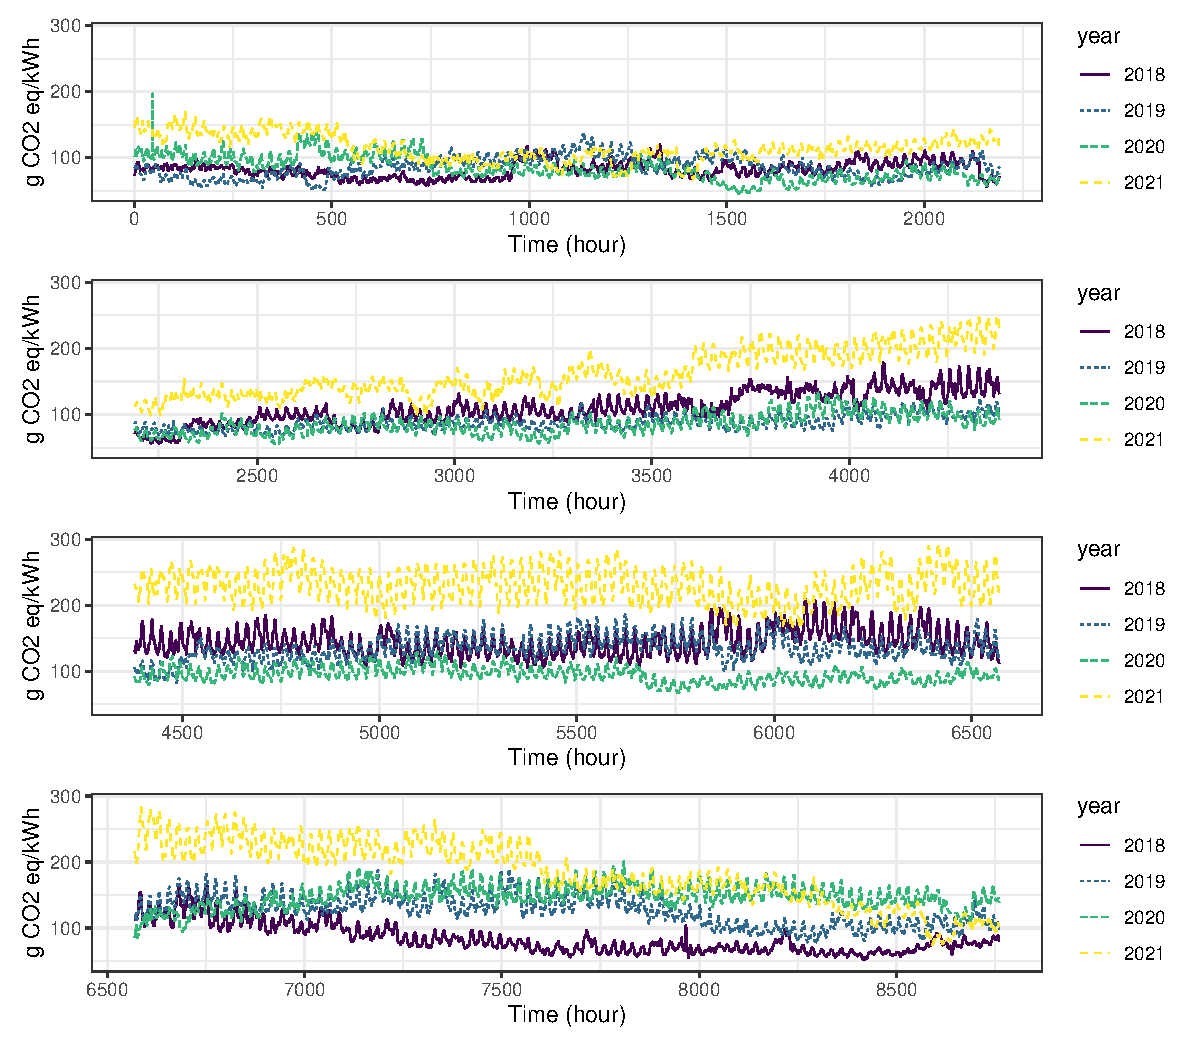
\epsfig{file = images/co2_emissions_sp.pdf, width = \textwidth}}
  \caption{São Paulo's hour by hour grid emissions for the years 2018, 2019, 2020 and 2021.}
  \label{fig:co2_sp}
\end{figure}

The scenario of Seoul --- ilustrated in Figure~\ref{fig:co2_seoul} --- represents a location with low presence of renewables: most of the electricity demand is supplied by carbon intensive sources as coal and gas. The small variation between the hours can be justified by the usage of PV panels, as when the sun starts shining they produce power and the emissions are reduced.


\begin{figure}[H]
  \centering
  {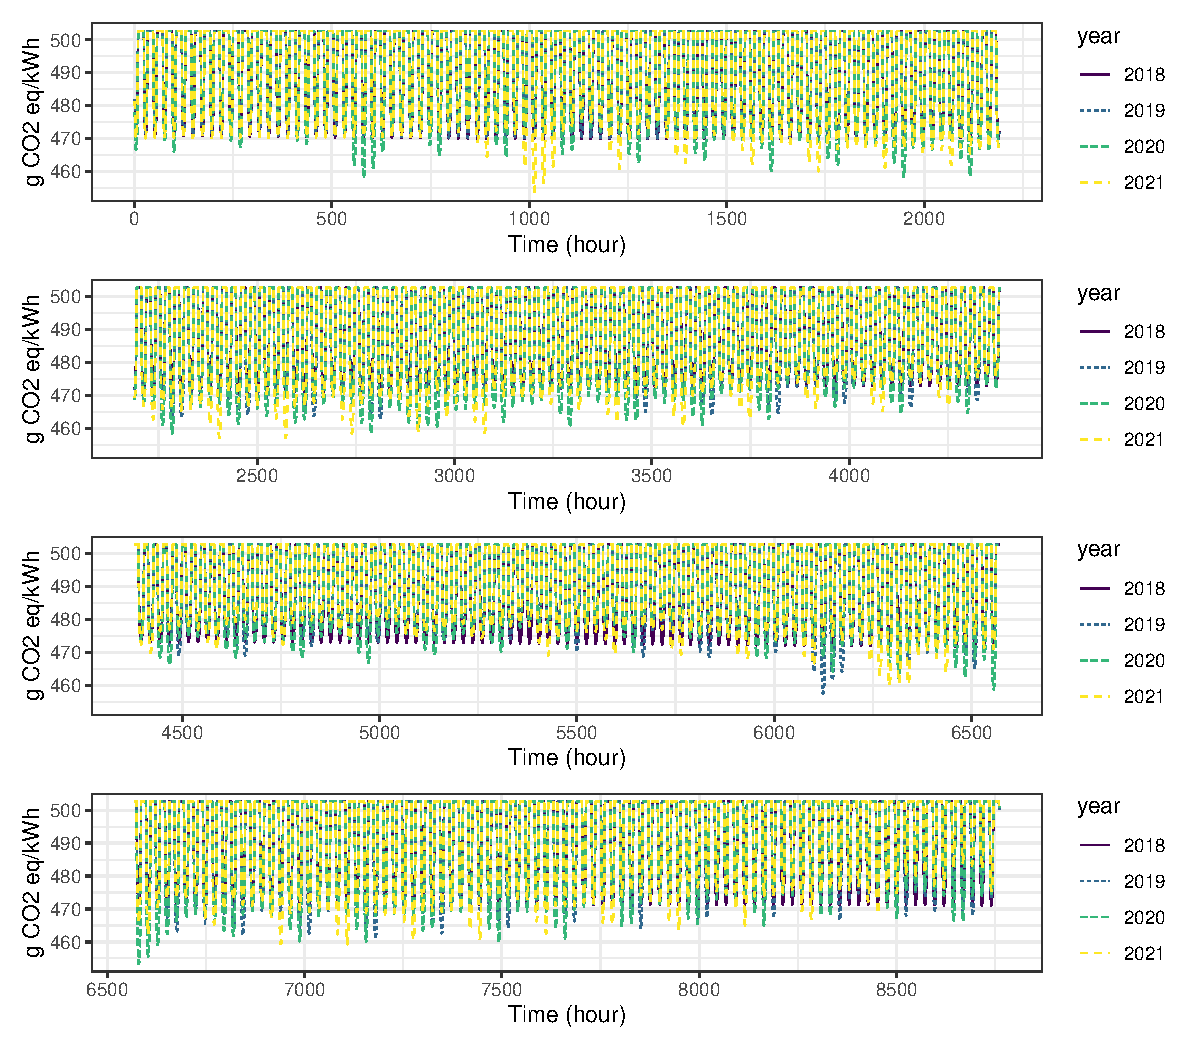
\epsfig{file = images/co2_emissions_seoul.pdf, width = \textwidth}}
  \caption{Seoul's hour by hour grid emissions for the years 2018, 2019, 2020 and 2021.}
  \label{fig:co2_seoul}
\end{figure}




\subsubsection{Results}

\paragraph{Intermittency of renewable sources}

Table~\ref{tab:co2_10y} presents the results in terms of \ch{CO2} emissions for the renewable infrastructure that included both PV panels and wind turbines, and in Table~\ref{tab:co2_10y_pv_only} only PV panels are considered.


\begin{table}[H]
  \caption{Emissions (in kt \ch{CO2}-eq) for the different scenarios --- renewable infra has PV panels and WT} \centering
    \label{tab:co2_10y}
      \begin{tabular}{|l|r|r|}        
        \hline        
        \textbf{Sizing Scenario} &  \textbf{Emissions } & \textbf{Diff. to baseline (\%) } \\
        \hline        
        Optimal sizing 2010 - 2019  &       301.931 & - \\
        \hline     
        Average irrad. and wind speed  1980 - 2009  &      342.584 &  11.9 \\
        \hline
        Median irrad. and wind speed  1980 - 2009  &      340.784 &   11.4 \\
        \hline        
      \end{tabular}      
    \end{table}

 \begin{table}[H]   
  \caption{Emissions (in kt \ch{CO2}-eq) for the different scenarios --- renewable infra only have PV panels} \centering

   \label{tab:co2_10y_pv_only}
  
      \begin{tabular}{|l|r|r|}        
        \hline
        \textbf{Sizing Scenario} &  \textbf{Emissions } & \textbf{Diff. to baseline (\%) } \\
       \hline        
        Optimal sizing 2010 - 2019       &       408.767 &  -       \\
        \hline     
        Average irradiation 1980 - 2009  &       414.956 &  1.49    \\
        \hline
        Median irradiation  1980 - 2009  &       422.928 &  3.35   \\
        \hline        
      \end{tabular}
      
    \end{table}

    

\paragraph{Fine-grain values of grid emission data (hour by hour)}

Table~\ref{tab:co2_grid_granularities_years} presents the increase in \ch{CO2} emissions (relative value in percent) of not having access to the fine-grain value of \ch{CO2} emissions (as hour by hour values).


\begin{table}[H]

  \caption{Difference in total emissions (tons of \ch{CO2}) between using avg. co2 of the year vs co2 per hour for the different years. Values greater than zero represents that using co2 values per hour increased the total emissions.}\label{tab:co2_grid_granularities_years} \centering

  \begin{tabular}{|l|r|r}
    \hline
    
  \textbf{Year} &   \textbf{Difference (\%) in \ch{CO2} emissions} \\
  \hline
  2018 &   0.34 \\
  \hline
  2019 &   0.59 \\
  \hline
  2020 &   0.18 \\
  \hline
  2021 &   0.74 \\
  \hline

\end{tabular}  
\end{table}


\section{Scheduling flexibility to reduce \ch{CO2} emissions}
\label{sec:flexibility}

\subsection{Updates in the model}

Suppose that we have the flexibility to delay $\alpha$ percent of workload up to $\beta$ time slots. We need two new variables to model this new feature: $alloc^d_k$ that represents the workload allocated to the data center $d$ that will start executing at the time slot $k$; and $delay_{k,i}^d$, which represents the workload of data center $d$ that can be delayed from time slot $k$ up to $\beta$ time slots ($i$ is the index of list of size $\beta$ for the delayed workload).

This feature also requires new restrictions. Equation~\eqref{eq:alpha} models the flexibility of allowing $\alpha$ percent of the workload to be delayed, where $W_k$ is the input that represents the total CPU cores demand to execute the workload at time slot k.


\begin{equation} \label{eq:alpha}
   \sum_{d=1}^D  \sum_{i=1}^{\beta} delay_{k,i}^d \leq  \alpha   \times W_k
\end{equation}


Equation~\eqref{eq:beta} models the flexibility to delay the workload up to the next $\beta$ time slots and ensure that all the workload will be executed:


\begin{equation} \label{eq:beta}
       \sum_{d=1}^D    (  alloc_k^d +    \sum_{i=1}^{\beta} delay_{k,i}^d  ) = W_k  
     \end{equation}

The allocated workload at a time slot k, and the delayed workloads from the previous k - $\beta$ time slots need to respect the data center servers CPU core capacity. Equation ~\eqref{eq:beta_capacity} models this restriction. 

\begin{equation} \label{eq:beta_capacity}
\sum_{d=1}^D    (  alloc_k^d  +    \sum_{i=k-\beta}^{k-1} delay_{  i ,  k-i  }^d  )  \leq C_d 
\end{equation}

\subsection{Experiments}

\subsubsection{Settings}

The cloud infrastructure, the workload, grid emissions, and the execution environment are the same as in Section  \ref{sec:settings_ccgrid}. In order to evaluate only the impact of the flexibility of the scheduling in reducing the carbon emissions, all the other parameters are fixed: workload, solar irradiation (average from 1980 to 2019), wind speed (average from 1989 to 2019) area of PV panels and the capacity of the batteries, number of wind turbines, power consumption of servers and network devices, and so on. We will present an evaluation for delaying 10\% up to 50\% of the workload --- $\alpha$ values of 0.1, 0.2, 0.3, 0.4 and 0.5 --- for the period of one hour up to one week --- $\beta$ values of 1h, 6h, 12h, 24h, 48h, 96h, 120h.

\subsubsection{Results}

The results of the experiments in terms of reduction of \ch{CO2} emissions are presented in Table \ref{tab:flex_scheduling}.

\begin{table}[h]
  \caption{Reductions of total carbon emissions ( \% ) in comparison to the scenario where is not possible to delay the workload.}\centering
       \label{tab:flex_scheduling}
\begin{tabular}{|l|r|r|r|r|r|r|r|r|r|}
\hline
\textcolor{black} {$\alpha$}, \textcolor{black}{$\beta$} &   \textcolor{black}{\textbf{ 1 h }} &  \textcolor{black}{\textbf{ 12 h }} &  \textcolor{black}{\textbf{ 24 h }} &  \textcolor{black}{\textbf{ 48 h }}  &   \textcolor{black}{\textbf{ 72 h}} &   \textcolor{black}{\textbf{ 96 h}} &   \textcolor{black}{\textbf{ 120 h }} &   \textcolor{black}{\textbf{ 144 h}} &   \textcolor{black}{\textbf{ 168 h}} \\ 
     \hline
 \textcolor{black}{ \textbf{10.0 \%}}   &  0.46 &  2.59 &  3.14 &  3.48 &  3.66 &  3.76 &  3.81 &  3.85 &  3.85 \\ 
\hline
 \textcolor{black}{ \textbf{20.0 \%}}   &  0.84 &  3.4 &  3.85 &  4.11 &  4.21 &  4.21 &  4.21 &  4.22 &  4.22 \\ 
\hline
 \textcolor{black}{ \textbf{30.0 \%}}   &  1.15 &  3.71 &  4.07 &  4.25 &  4.25 &  4.26 &  4.26 &  4.27 &  4.27 \\ 
\hline
 \textcolor{black}{ \textbf{40.0 \%}}   &  1.42 &  3.89 &  4.15 &  4.25 &  4.26 &  4.27 &  4.28 &  4.28 &  4.29 \\ 
\hline
 \textcolor{black}{ \textbf{50.0 \%}}   &  1.65 &  4.01 &  4.22 &  4.26 &  4.27 &  4.28 &  4.29 &  4.3 &  4.3 \\ 
\hline
\end{tabular}
\end{table}




\section{ Monetary costs of reducing the carbon emissions}
\label{sec:costs}
On the previous sections we showed the results only in terms of the environmental impact of the cloud operation, now we will present the results in terms of monetary costs (in dollars) of operating the cloud platform and how much would it costs for the DC operator to reduce their environmental impact. This is also an important aspect, as the decision-makers wants their business to be lucrative.

\subsection{Updates in the model}

To perform this new analysis, we need some modification in our modeling. The first modification regards buying electricity from the regular grid, and it is modeled by Equation~\eqref{eq:pricegrid}, where $costGrid^d$ is an input that represents the costs of buying electricity at each location (in dollars per kWh). 

\begin{equation} \label{eq:pricegrid}
 PriceGrid^d_k = Pgrid^d_k \times costGrid^d
\end{equation}

To measure the price of the electricity of the renewable sources, we can use the metric Levelized Cost of Energy (LCOE) \cite{nrel_economic_wt_1995}. This metric compares the total costs of manufacturing and operating the electricity infrastructure (for example the PV panel) with the total energy it can deliver in its life time, and the metric is in form of costs per unit of electricity generated ---  \$ per kWh.

Similar to the \ch{CO2} emissions of renewable sources, the price will also be different per location, as the total amount of irradiation received and wind speed differs.

Equation~\eqref{eq:pricepv} models the costs of consuming energy from the solar panels, where $PVLCOE^d$ represents the specific LCOE at the location of data center $d$ (in dollars per kWh).

\begin{equation} \label{eq:pricepv}
  PricePV^d_k = PPV^d_k \times PVLCOE^d
\end{equation}


For the wind turbines, we also use the LCOE to compute its price, and Equation~\eqref{eq:pricewt} models the costs of using energy from the WT, where $WTLCOE^d$ represents the specific LCOE at the location of data center $d$ (in dollars per kWh).


\begin{equation} \label{eq:pricewt}
  PriceWT^d_k = PWT^d_k \times WTLCOE^d
\end{equation}

For the batteries, the metric Levelized Cost of Storage (LCOS) is similar to the LCOE, and it represents the cost per unit of energy discharged ( dollars per kWh or MWh) that takes into account its whole life cycle: calendar and cycle life, Max Depth of Discharge limitations, and costs from operation and maintenance \cite{battery_lcos_2022}.  Equation~\eqref{eq:pricebat} models the costs of the energy used from the batteries using its LCOS as input ($BatLCOS$ in dollars per kWh of electricity discharged).

\begin{equation} \label{eq:pricebat}
   PriceBat^d_k = Pdch^d_k \times BatLCOS
\end{equation}



We can also modify our objective function to minimize the price of operating the cloud platform instead of its environmental impact, and Equation~\eqref{eq:objective_price} model this new objective.

\begin{equation} \label{eq:objective_price}
\text{minimize }\sum_{k=0}^{K-1} \sum_{d=1}^D PriceGrid^d_k  + PriceBat^d_k + PricePV^d+ PriceWT^d_k
\end{equation}


\subsection{Experiments}

\subsubsection{Settings}

The cloud infrastructure, the workload, grid emissions, and the execution environment are the same as in Section  \ref{sec:settings_ccgrid}.

For the price of solar panel electricity, we use the tool ``Comparative Photovoltaic Levelized Cost of Energy Calculator'' from the National Renewable Energy Laboratory of the USA \cite{pv_lcoe_calc} --- version 2.0.0 of August 2021. This tool provide a detailed cost model for many parts of the PV panel, and the default values are adequate. For reproducibility purposes, Table \ref{tab:parameters_pv_LCOE} lists the values of the parameters used, and the only differences between the default values were for the parameters Service life, Performance Efficiency, and the Energy yield (that depends on the location where the PV module is installed). For the latter, the following values where considered: Canberra = 1934.03 ; Seoul  = 1648.08; Paris = 1346.32 ; Virginia = 1737.38; Dubai =  2215.17; Singapore = 1549.23; Pune =  2125.62 ; Johannesburg = 2238.52; and São Paulo =  1904.66.

\begin{table}[h]
  
  \caption{Parameters used in the LCOE PV calculator}\label{tab:parameters_pv_LCOE} \centering

  \begin{tabular}{|l|r|}
    \hline    
    \textbf{Parameter name} &   \textbf{Value} \\
    \hline
    Cell technology & mono-SI  \\
    \hline
    Package type  & glass-polymer backsheet \\
    \hline
    System type  & fixed tilt, utility scale \\
    \hline
    Inverter loading ration  & 1.5 \\
    \hline
    Front layer cost (USD/m²)   &  3.5 \\
    \hline
    Cell  cost (USD/m²)   &  22.20 \\
    \hline
    Back layer cost (USD/m²)   & 2.40 \\
    \hline
    Non-cell module cost (USD/m²)   &  13.60 \\
    \hline
    Extra component cost (USD/m²)   &  0 \\
    \hline
    Operations and Maintenance cost  (USD/kWDC/year)   &  3.5 \\
    \hline  
    Balance of system cost,power-scaling  (USD/W)   &  0.2 \\
    \hline  
    Balance of system cost,area-scaling  (USD/m²)   &  53.38 \\
    \hline  
    Performance Efficiency (\%) & 15.0  \\
    \hline
    Energy yield (kWh/kWDC) & specific per location \\
    \hline
    System degradation rate (\%/year)  & 1.0 \\
    \hline
    Service life (years) & 30 \\
    \hline
    Discount rate & 6.3 \\
    \hline
    

  \end{tabular}  
\end{table}


For computing the LCOE (dollars per MWh) of wind turbines, we also used the modeling from NREL~\cite{nrel_wt_costs_2021}. Equations~\eqref{eq:wt_lcoe} represents how to calculate the LCOE for WT, where CapEx is the capital expenditures (dollars per kilowatt) --- represents the initial investment cost in the infrastructure, OpEx is the operation expenditures (dollars per kilowatt per year), FCR is the fixed charge rate (\%) --- the amount of revenue per dollar of investment that must be collected annually from customers to pay the carrying charges on that investment, such as return on debt and equity, income and property tax, book depreciation and insurance ~\cite{nrel_economic_wt_1995}. We used the default values for a Distributed Single-Turbine (Large): Capex = 3540; Fcr = 5.42; OpEx = 35. For the net annual energy production (in MWh/MW/year), it also depends on the location where the wind turbine is installed: Canberra = 1138.5; Seoul  = 829.57; Paris = 2065.38 ; Virginia = 1289.12; Dubai = 1217.64; Singapore = 754.0; Pune =  869.19 ; Johannesburg = 1143.32; and São Paulo = 881.95.

\begin{equation} \label{eq:wt_lcoe}
  LCOE_{wt} = \frac{ (CapEx \times FCR) + OpEx}{ \frac{AEP_{net}}{1000}   }
\end{equation}

For the batteries, the metric Levelized Cost of Storage (LCOS) is similar to the LCOE, and it can represents how much it costs to discharge energy of the battery considering all the costs in its lifetime. We used values from a technical report of the US Department of Energy \cite{battery_lcos_2022}, where each kilowatt hour of energy discharged has a price of 20 cents. Finally, Table \ref{tab:price_electricity_sources} presents the cost in dollars per kWh of using the electrical grid, PV panels and wind turbines.

\begin{table}[h]
  
  \caption{Price of different sources of energy (USD per kWh) at each location. Source for the grid electricity prices: Petrolprices.org.  }\label{tab:price_electricity_sources} \centering
  
  \begin{tabular}{|l|r|r|r|}
  \hline    
  \textbf{Location} &   \textbf{Grid} & \textbf{PV} & \textbf{WT} \\
  \hline
  Johannesburg & 0.074 & 0.0385 &  0.1984   \\
  \hline
  Pune      &  0.104   & 0.0406 & 0.2610    \\
  \hline
  Canberra  & 0.331    &  0.0445 & 0.1993   \\
  \hline
  Dubai   & 0.101      & 0.0390 &   0.1863  \\
  \hline
  Singapore & 0.272    & 0.0557 & 0.3009    \\
  \hline     
  Seoul      & 0.092   & 0.0525 & 0.2735    \\
  \hline
  Virginia   & 0.150   &  0.0498 &  0.1760  \\
  \hline
  São Paulo  & 0.144   &  0.0453 & 0.2572   \\
  \hline 
  Paris      & 0.340   &  0.0643 & 0.1098   \\
  \hline  

\end{tabular}
\end{table}

\subsubsection{Results}

Table~\ref{tab:total_price} illustrates the total costs (in dollars) for the data center operator considering multiple scenarios. The \textit{Minimum Costs} scenario refers to solving the LP using the objective of Equation~\eqref{eq:objective_price}; the \textit{Minimum \ch{CO2}} refers to solving the LP using the objective of Equation~\eqref{eq:FPALL}, and for both cases the reader will find in parentheses the configuration of the renewable infrastructure used.; and \textit{Only grid} represents the case where there is no renewable infrastructure in the DCs and they only use power from the local electricity grid.


\begin{table}[h]
  
  \caption{Total costs (millions of \$) for different scenarios }\label{tab:total_price} \centering
  \begin{tabular}{|l|r|}
   \hline  
  \textbf{Scenario} &   \textbf{Total costs (millions of \$)} \\    
  \hline
  Minimum cost (PV + WT+ Bat + grid) & 47.73    \\
  \hline
  Minimum cost (PV + Bat + grid)      & 50.87     \\ 
  \hline    
  Only grid   & 75.39                             \\
  \hline
  Minimum \ch{CO2} (PV + Bat + grid) & 78.92       \\
  \hline
  Minimum \ch{CO2} (PV +WT+  Bat + grid) & 118.31 \\
  \hline
  
\end{tabular}  
\end{table}

In order to allow a better evaluation of the environmental impact of minizing the monetary costs, the emissions of the evaluated scenarios (in tons of \ch{CO2} eq.) are presented in Table~\ref{tab:total_co2_scenarios_costs}.

\begin{table}[h]

  \caption{Total emissions (tons of \ch{CO2} eq. for different scenarios }\label{tab:total_co2_scenarios_costs} \centering
  
  \begin{tabular}{|l|r|}
  \hline
  \textbf{Scenario} &   \textbf{Total emissions (tons of \ch{CO2} eq)} \\
  \hline
  Minimum \ch{CO2} (PV + WT +  Bat + grid)  & 24373.88 \\
  \hline
  Minimum \ch{CO2} (PV +  Bat + grid)  & 37778.79 \\    
  \hline
  Minimum cost (PV + WT+ Bat  + grid) &  129713.08 \\
  \hline
  Minimum cost (PV + Bat  + grid)   & 131597.65 \\
  \hline
  Only grid & 201211.31  \\
  \hline
\end{tabular}  

\end{table}

Finally, Figures ~\ref{fig:pv_co2_costs},  ~\ref{fig:bat_co2_costs}, and ~\ref{fig:wt_co2_costs}, shows the difference in the renewable infrastructure sizing when the objective function is to minimize the costs and the carbon emissions of the cloud federation operation.

\begin{figure}[H]
  \centering
  {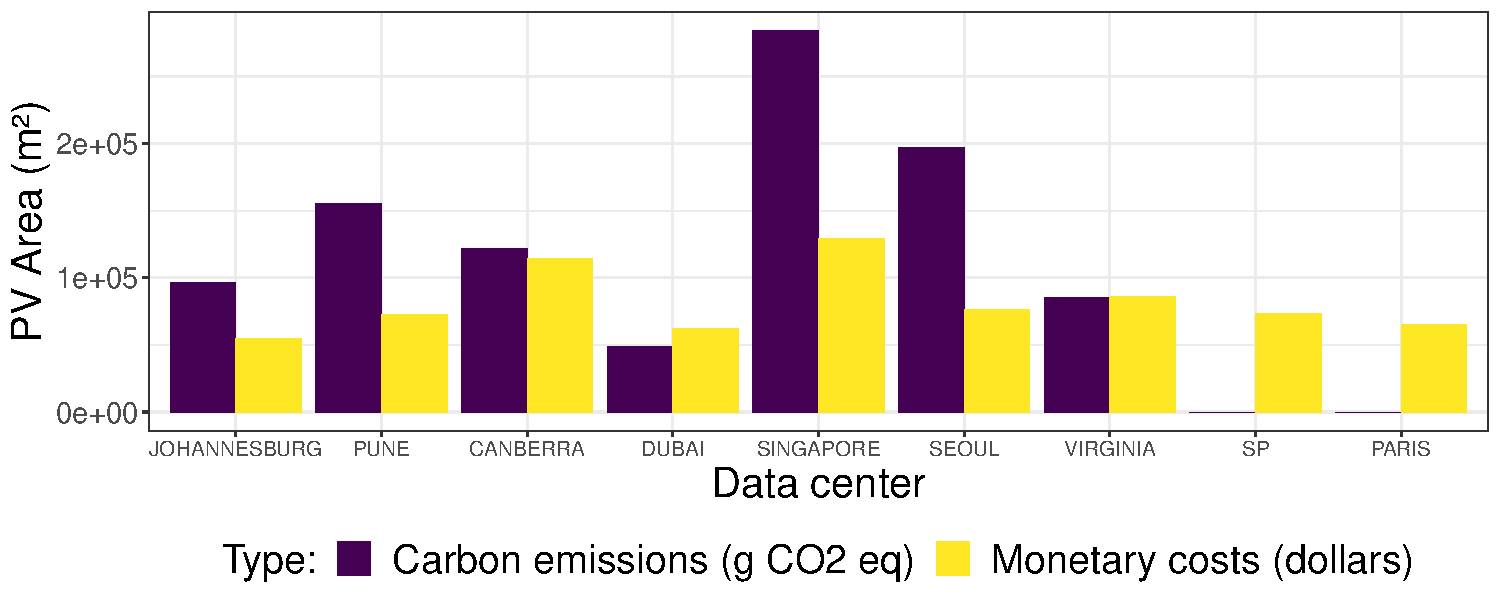
\epsfig{file = images/pv_sizing_co2_costs.pdf, width = .8\textwidth}}
  \caption{PV Area to minimize costs in comparison to minimizing carbon emissions. }
  \label{fig:pv_co2_costs}
\end{figure}


\begin{figure}[H]
  \centering
  {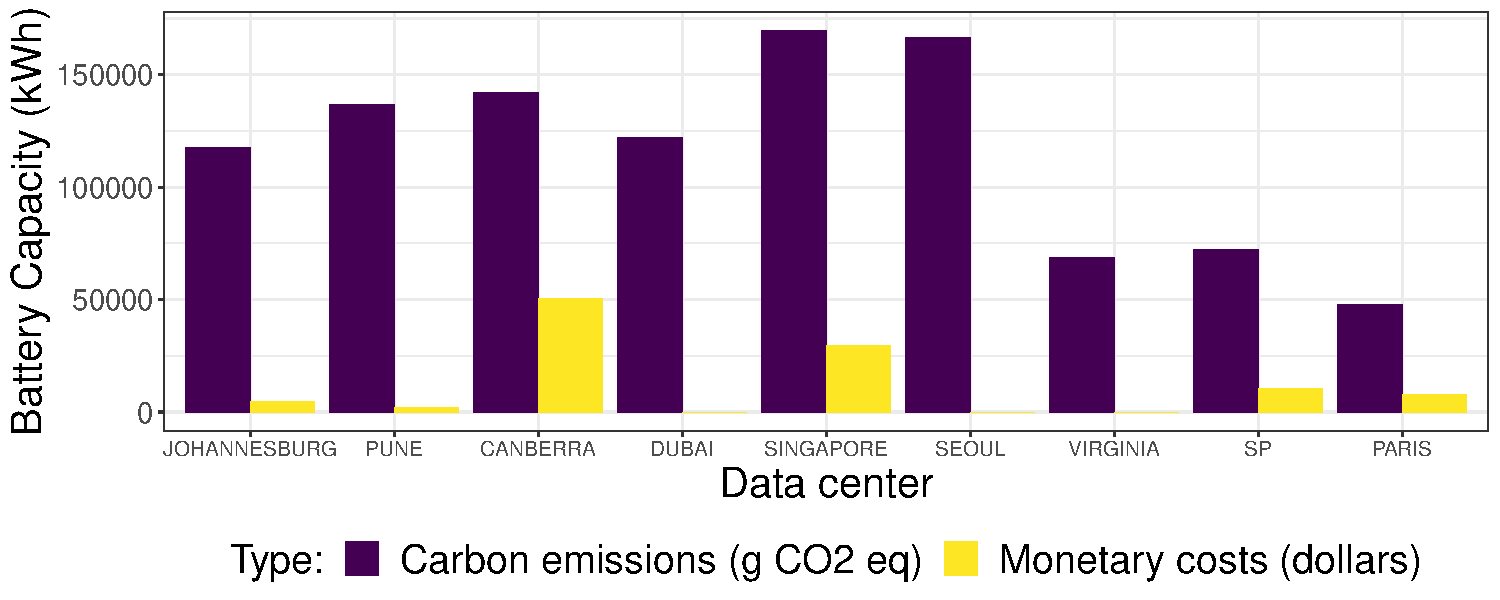
\epsfig{file = images/bat_sizing_co2_costs.pdf, width = .8\textwidth}}
  \caption{Battery capacity to minimize costs in comparison to minimizing carbon emissions.  }
  \label{fig:bat_co2_costs}
\end{figure}

\begin{figure}[H]
  \centering
  {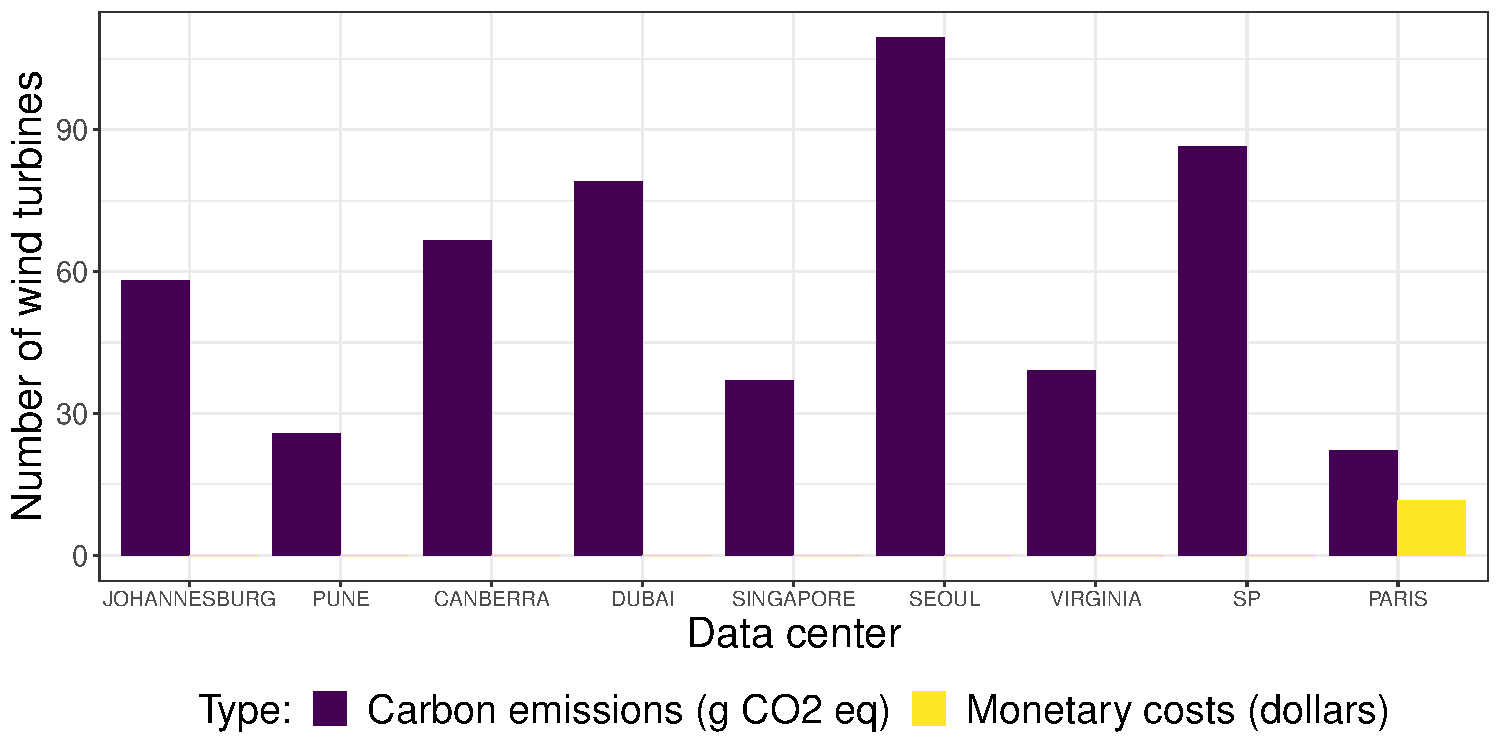
\epsfig{file = images/wt_sizing_co2_costs.pdf, width = .8\textwidth}}
  \caption{Number of wind turbines  to minimize costs in comparison to minimizing carbon emissions.}
  \label{fig:wt_co2_costs}
\end{figure}


\section{Adding or replacing servers considering new generations }
\label{sec:new_servers}
In this section we show the necessary modifications in our modeling to evaluate the decision of manufacturing servers from new generations to match the cloud workload demand, considering that the servers also emits \ch{CO2} during its life time. It is assumed a long-term operation of the cloud federation (10 years for example) and that new servers will be launched during the life time of the cloud data centers. The decision-maker of the cloud federation will determine to add new servers to operate with the older ones from previous generations or to replace them.

\subsection{Updates in the model}

To model this approach, two new variables were created: $NS^d$, that represents the number of new servers to manufacture at data center $d$; and $REP_{gen}^d$, number of servers of the generation $gen$ to replace at data center $d$. For replacing the servers from previous generations, it is considered that the data center computational capacity in number of CPU cores cannot decrease, that is, the total of the number of CPU cores of the new servers needs to be greater or equal to the total number of CPU cores from the servers replaced. This constraint is modeled by Equation~\eqref{eq:dc_cpu_capacity}.

\begin{equation} \label{eq:dc_cpu_capacity}
 NS^d \times cpucores_{newgen} \geq \sum_{oldergen}  REP_{oldergen}^d \times cpucores_{oldergen}
\end{equation}

The number of servers replaced of a generation cannot be greater than the number of servers of this generation that exists in the DC ($ES_{gen}^d $). The value of  $ES_{gen}^d $ is extracted from the solution of the previous year. Equation~\eqref{eq:rep_only_existing_servers} models this constraint.

\begin{equation} \label{eq:rep_only_existing_servers}
 REP_{gen}^d \leq ES_{gen}^d 
\end{equation}


Given that a data center may have servers of different generations, it is also necessary to update the models regarding the workload execution and the power consumption. Now we have a variable $w_{k,gen}^d$ that represents the workload that is executed on the servers of a generation $gen$ at the data center $d$ during time slot $k$. We have two constraints for this variable: one for the servers that already exists in the DC, and another for the new servers that will be manufactured in the DC. Equation~\eqref{eq:workload_gen} models this constraint.


\begin{equation} \label{eq:workload_gen}
w_{k,gen}^d \leq   \left\{ 
  \begin{array}{ c l }
    (ES_{gen}^d - REP_{gen}^d) \times cpucores_{gen}  & \quad \textrm{if server from older generation  }     \\
     NS^d \times cpucores_{gen}   & \quad \textrm{if server from new generation  }      \\
    
  \end{array}
\right.
\end{equation}

Equation~\eqref{eq:wkgen} models the constraint that all the workload must be executed, and that it can be run in any generation of the servers.

\begin{equation} \label{eq:wkgen}
    w_k = \sum_{T_i|r_i\leq k\Delta t<r_i+p_i} c_i = \sum_d \sum_{gen} w_{k,gen}^d
\end{equation}

We also assume that the workload is classified in two categories: services that are mandatory tasks that execute in the DCs, and batch tasks that can execute in any of the DCs. This assumptions represents the modern workload of cloud platforms and also avoid allocating all the workload to the DC with the lowest-carbon intensity grid and only adding and replacing servers on this DC. To model the classification of the workload in two categories, we need a new parameter $\gamma$ that represents the ratio of tasks that are of the service type (and 1 - $\gamma$ tasks are of the batch type) executed at each data center $d$. Equation~\eqref{eq:workload_category} models this restriction.

\begin{equation} \label{eq:workload_category}
 \sum_{gen}  w_{k,gen}^d \geq  w_k \times \gamma^d
\end{equation}


Equation~\eqref{eq:power_servers_gen} presents the new modeling of the power consumption for all the servers of different generations at a DC $d$, and Equation~\eqref{eq:power_cons_gen} models the power consumption of the DC (including the costs of the intra-network equipment and the cooling devices).


\begin{equation} \label{eq:power_servers_gen}
   PServers^d  =  \big(   \sum_{gen} ES_{gen}^d \times  Pidle_{gen}^d + w^d_{k,gen}  \times  Pcore_{gen} \big)
\end{equation}


\begin{equation} \label{eq:power_cons_gen}
   P^d_k  = PUE^d \times \big(  Pintranet^d + PServers^d\big)
\end{equation}


Regarding the carbon footprint of the servers, it is assumed that it is amortized over the server life time and the LP considers the annual value. For example, if manufacturing a server emits 800 kg of \ch{CO2} eq. and its expected life time of 4 years, 25\% (200 kg of \ch{CO2} eq.) of its manufacturing emissions will be accounted on the 1st year of operation, other 25\% at the second year and so on. After the fourth year, the server can still remain in the cloud plataform, and its carbon emissions will come only from the power consumption --- all the carbon emissions from manufacturing has been amortized.  On the other hand, if the server is replaced at the second year of operation, the 75\% remaining of its emissions from manufacturing will also be taken into account. Equation~\eqref{eq:co2_new_servers} illustrates the footprint of building additional servers at a given data center $d$, where $serversCO2$ is an input with the total \ch{CO2} emitted from manufacturing the server, and $\epsilon$ the share of the emissions by year ---  $\epsilon$ is equal to 0.25 on the previous example.


\begin{equation} \label{eq:co2_new_servers}
FPns^d = NS^d \times ( serversCO2 \times \epsilon)	
\end{equation}


Equation~\eqref{eq:co2_rep_servers} illustrates the footprint of replacing servers from previous generations at a given data center $d$, where $repCO2_{gen}$ is the emissions (in kg of \ch{CO2} eq) from replacing the old servers that depends on the server age ($age_{gen}$) in years. The function that computes the value of  $repCO2_{gen}$  is defined in Equation~\eqref{eq:amortizedCO2}. 

\begin{equation} \label{eq:co2_rep_servers}
FPrep^d = \sum_{gen} REP_{gen}^d  \times repCO2_{gen}
\end{equation}


\begin{equation} \label{eq:amortizedCO2}
repCO2_{gen} =  \left\{ 
  \begin{array}{ c l }
    (1 - (age_{gen} * \epsilon)) \times serverCO2   & \quad \textrm{if $age_{gen}$}  <  \textrm{expected life time}      \\
    0     & \quad  \textrm{otherwise}   \\
  \end{array}
\right.
\end{equation}


We also have the carbon footprint of the servers that were manufactured in previous years. Equation~\eqref{eq:co2_existing_servers} illustrates the emissions of the \textbf{e}xisting \textbf{s}ervers where $esCO2_{gen}$ represents the emissions of operating the server of the generation $gen$ during that year (in kg of \ch{CO2} eq) and its value is computed by the function in Equation~\eqref{eq:serverCO2}.


\begin{equation} \label{eq:co2_existing_servers}
FPes^d = \sum_{gen} ( ES_{gen}^d - REP_{gen}^d )  \times esCO2_{gen}
\end{equation}

\begin{equation} \label{eq:serverCO2}
esCO2_{gen} =  \left\{ 
  \begin{array}{ c l }
    \epsilon \times serverCO2   & \quad \textrm{if $age_{gen}$}    < \textrm{expected life time}   \\
    0     & \quad \textrm{otherwise  } \\
  \end{array}
\right.
\end{equation}


Finally, Equation~\eqref{eq:new_obj_co2_servers} presents the new objective function of operating the cloud platform considering that new servers can be manufactured, and servers from previous generations can be replaced.

\begin{equation} \label{eq:new_obj_co2_servers}
\text{minimize }\sum_{k=0}^{K-1} \sum_{d=1}^D ( FPgrid^d_k +  FPpv^d_k + FPbat^d_k) + \sum_{d=1}^D   FPns^d + FPrep^d + FPes^d 
\end{equation}

It is assumed that the renewable infrastructure cannot change from one year to the other. Equations~\eqref{eq:low_bound_bat},  ~\eqref{eq:low_bound_pv} and ~\eqref{eq:low_bound_wt} model these constraints, where $lowboundbat^d$, $lowboundpv^d$ and $lowboundwt^d$ are the capacity of batteries, area of PVs and number of wind turbines, respectively, obtained from the sizing process.

\begin{equation} \label{eq:low_bound_bat}
Bat^d = lowboundbat^d
\end{equation}

\begin{equation} \label{eq:low_bound_pv}
A^d = lowboundpv^d
\end{equation}

\begin{equation} \label{eq:low_bound_wt}
WT^d = lowboundwt^d
\end{equation}


\subsection{Experiments}

\subsubsection{Settings}


We consider ten years of operation and seven generations of servers. Table~\ref{tab:servers_specs} lists the difference in terms of hardware characteristics, power consumption, and the carbon footprint of manufacturing each generation. For the \ch{CO2} of manufacturing the servers, the methodology from~\cite{gupta2022_ACT} is used, that presents how to compute the carbon footprint of servers considering the integrated circutis of  RAM, storage (HD and SSDs) and CPU.

\begin{table}[h]
  \small
  \caption{Servers specifications for different generations} \centering
  \label{tab:servers_specs} 
  \begin{tabular}{|l|r|r|r|r|r|r|}

  \hline
    
  \textbf{Years} & \textbf{CPU} &   \textbf{CPU Cores} & \textbf{P idle}  & \textbf{P Core} & \textbf{Nodes} & \textbf{kg \ch{CO2} eq.} \\
  \hline
    1    & Intel Xeon E5-2630 & 20 & 52 & 7.5 & 1 & - \\
  \hline
    2, 3 & Intel Xeon E5-2699 v3 & 36 & 40.1 & 6.3 & 1 & 577.2\\
  \hline
     4   & Intel Xeon E5-2698 V4 &  40 & 43.5 & 7.1375 & 1 & 569.4\\
  \hline
    5, 6 & Intel Xeon Platinum 8180 & 56 & 48.9 & 6.68 & 1 & 578.6\\
  \hline
    7, 8 & AMD EPYC 7742  & 64 & 66.1 & 2.71 & 1 & 587.2 \\
  \hline
    9    & AMD EPYC 7763 & 128 & 75.6 & 3 & 1    & 590.3 \\
  \hline
   10    & AMD EPYC 9654 & 192 & 126 & 3.65 & 1 & 614.9 \\
  \hline
\end{tabular}  
\end{table}

All the servers are based on the Dell R740 for the HD and SSD values (HD with 3.84 TB and SSD with 400GB), with same values for \ch{CO2} as in ~\cite{gupta2022_ACT} and they have 256 GB of RAM (16 modules of 16 GB DDR4 10 nm). For the CPU, the \ch{CO2} depends on the die are size and the processor size (in nanometers), and the respective values can be seen in Table~\ref{tab:cpu_specs}. For the first generation, it is considered that the server have been used more than its expected life time and all its \ch{CO2} footprint have been paid. Finnaly, it is considered that the servers have a expected life time of 4 years.

\begin{table}[h]
  \small
  \caption{CPU specifications in terms of die area and processor size. Source: x86guide.net} \centering
  \label{tab:cpu_specs} 
  \begin{tabular}{|l|r|r|}
   \hline

  \textbf{Model}  & \textbf{CPU die area (cm²)} & \textbf{Processor size (nm)} \\
  \hline
    Intel Xeon E5-2699 v3& 6.62  & 20  \\
  \hline
    Intel Xeon E5-2698 V4 & 4.56 & 14\\
  \hline
    Intel Xeon Platinum 8180 & 6.94 & 14\\
  \hline
    AMD EPYC 7742  & 5.92 & 7 \\
  \hline
    AMD EPYC 7763 & 6.45   & 7 \\
  \hline
    AMD EPYC 9654 & 8.66 & 5 \\
  \hline
\end{tabular}  
\end{table}


Two scenarios will be considered in the experiments. In the first, the LP is solved year by year and it only has access to the climate conditions, workload and server configuration of the current year. After the LP is solved for the year $x$, the results in terms of new servers manufactured and older ones replaced will be used as input to the year $x +1$. In the second scenario, the 9 years of operation are solved at once, therefore the LP has access to all the information about future workload, climate conditions and servers configurations. The first scenario represents an approach more realistic that has potential to be taken by the decision maker, considering that is hard to have accurate values for workload, climate conditions and servers configurations in the long term, and the second scenario is only used as baseline --- it represents the optimal solution.

\subsubsection{Results}

Figure \ref{fig:dc_evolution_year_by_year} presents the result of the DCs evolution when the decision is made year by year, that is, at each year the cloud-federation operator has information about the configurations of the current generation's server, and the decision is made to manufacture these new servers to add or to replace older ones. Figure \ref{fig:dc_evolution_optimal} presents the optimal solution, when all the information about the workload, servers specifications, climate conditions, is known in advance for the 10 years. We observe that the optimal solution make very few changes in the servers, because it knows in advance when is the right moment to add/replace the servers. However, in real-life the first approach where the decision is made year by year is more close to what the cloud-federation operator would do. Finally, in terms of total \ch{CO2} emissions, the optimal solution is 10\% better than the solution that only has information about the current year, as can be seen in Table~\ref{tab:emissions_sizing}.

\begin{figure}
\centering
  
  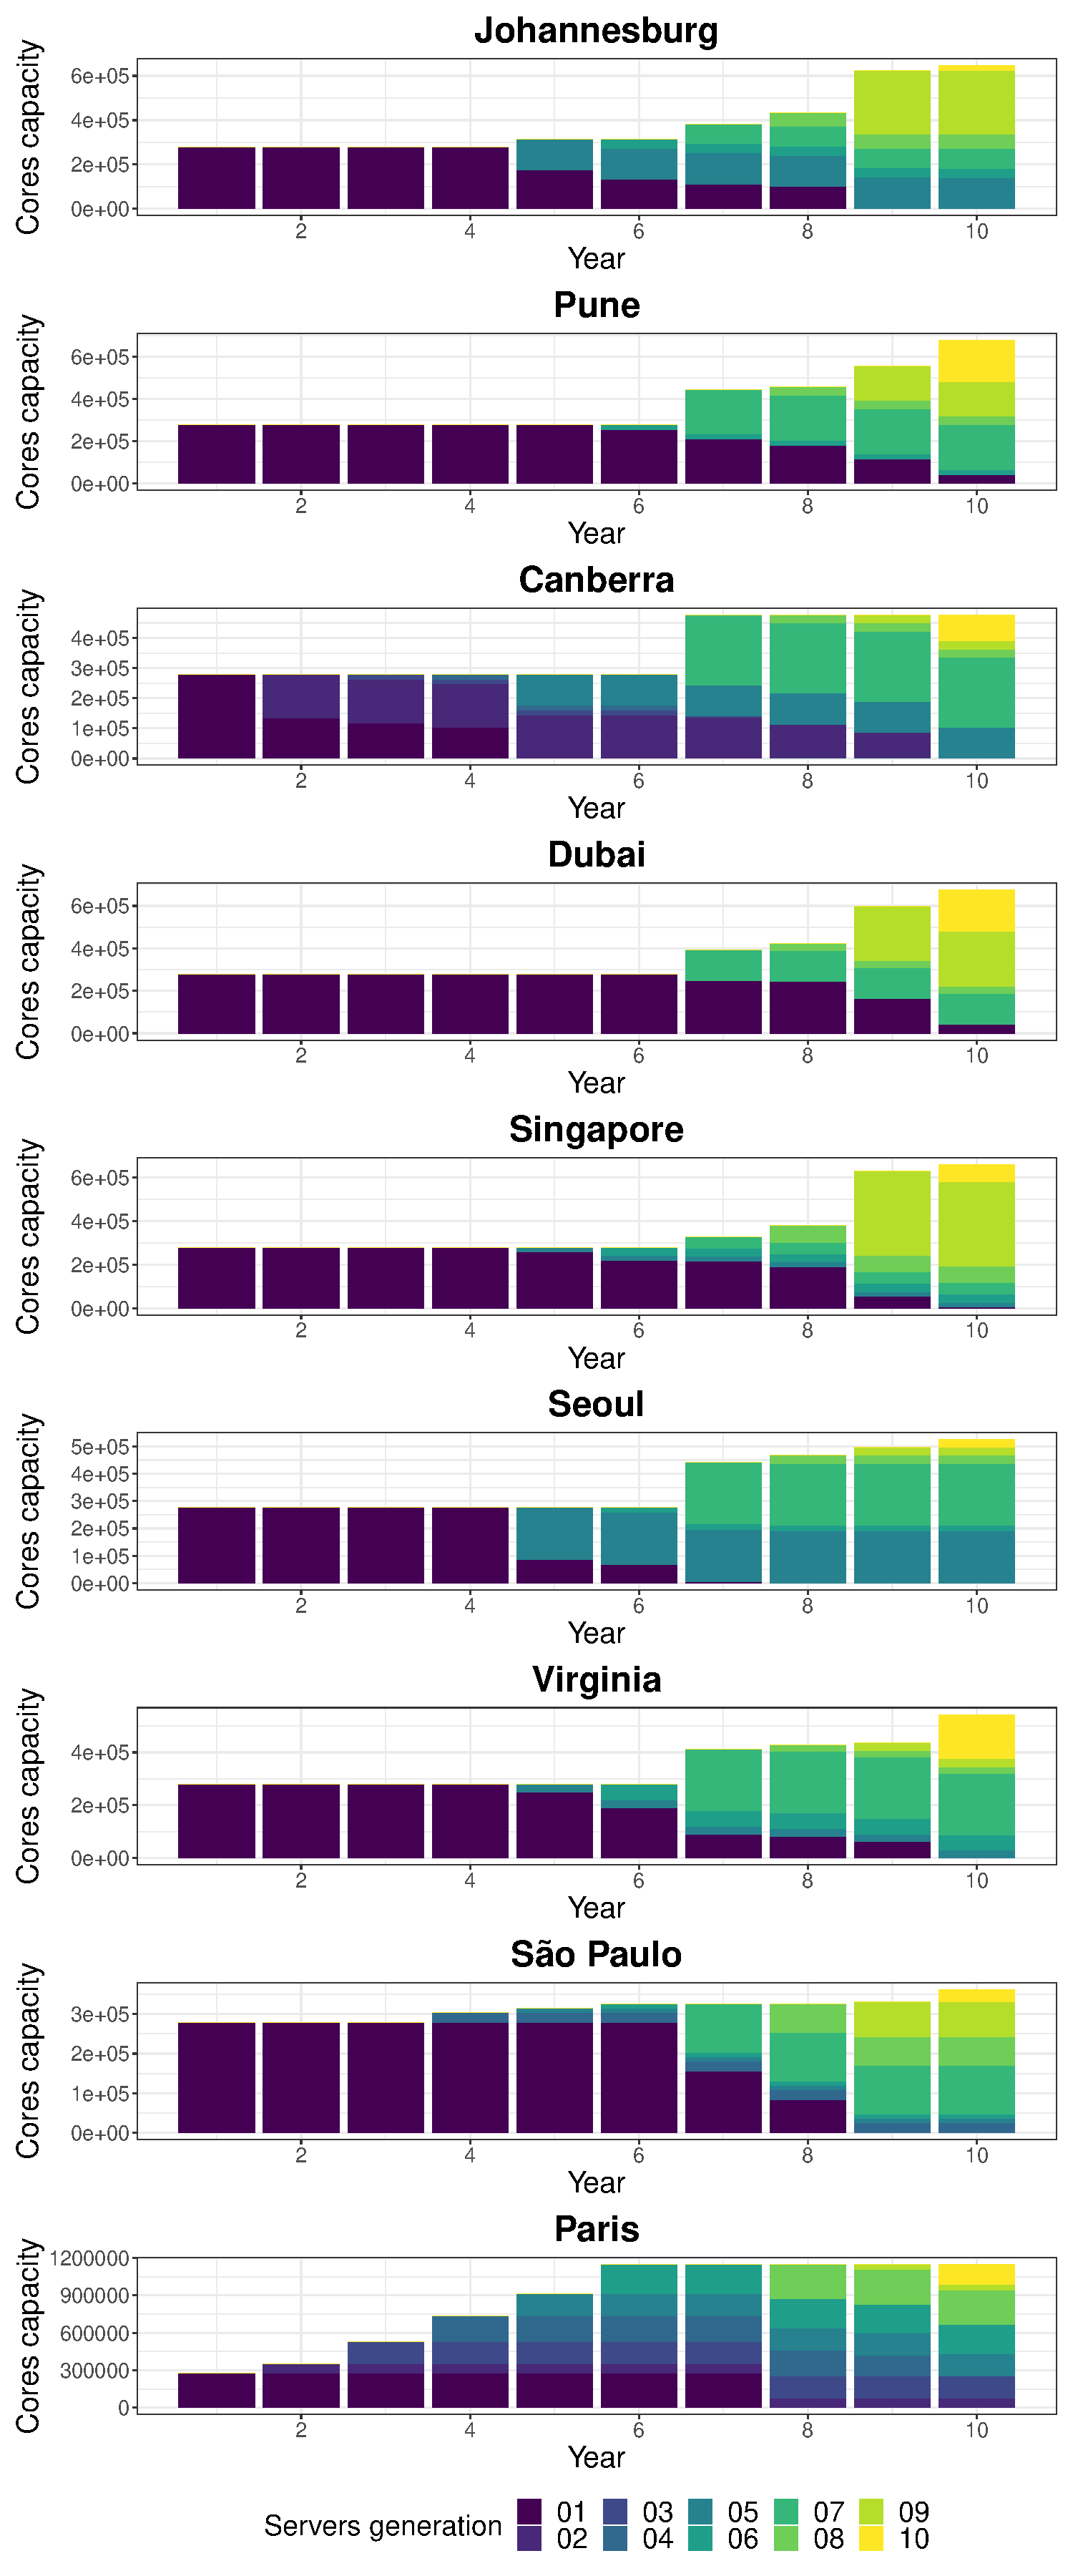
\includegraphics[width=\linewidth]{images/dc_evolution_year_by_year.pdf}
  \caption{Cloud federation evolution knowing only the information of the current year.}
  \label{fig:dc_evolution_year_by_year}
\end{figure}

\begin{figure}
\centering
  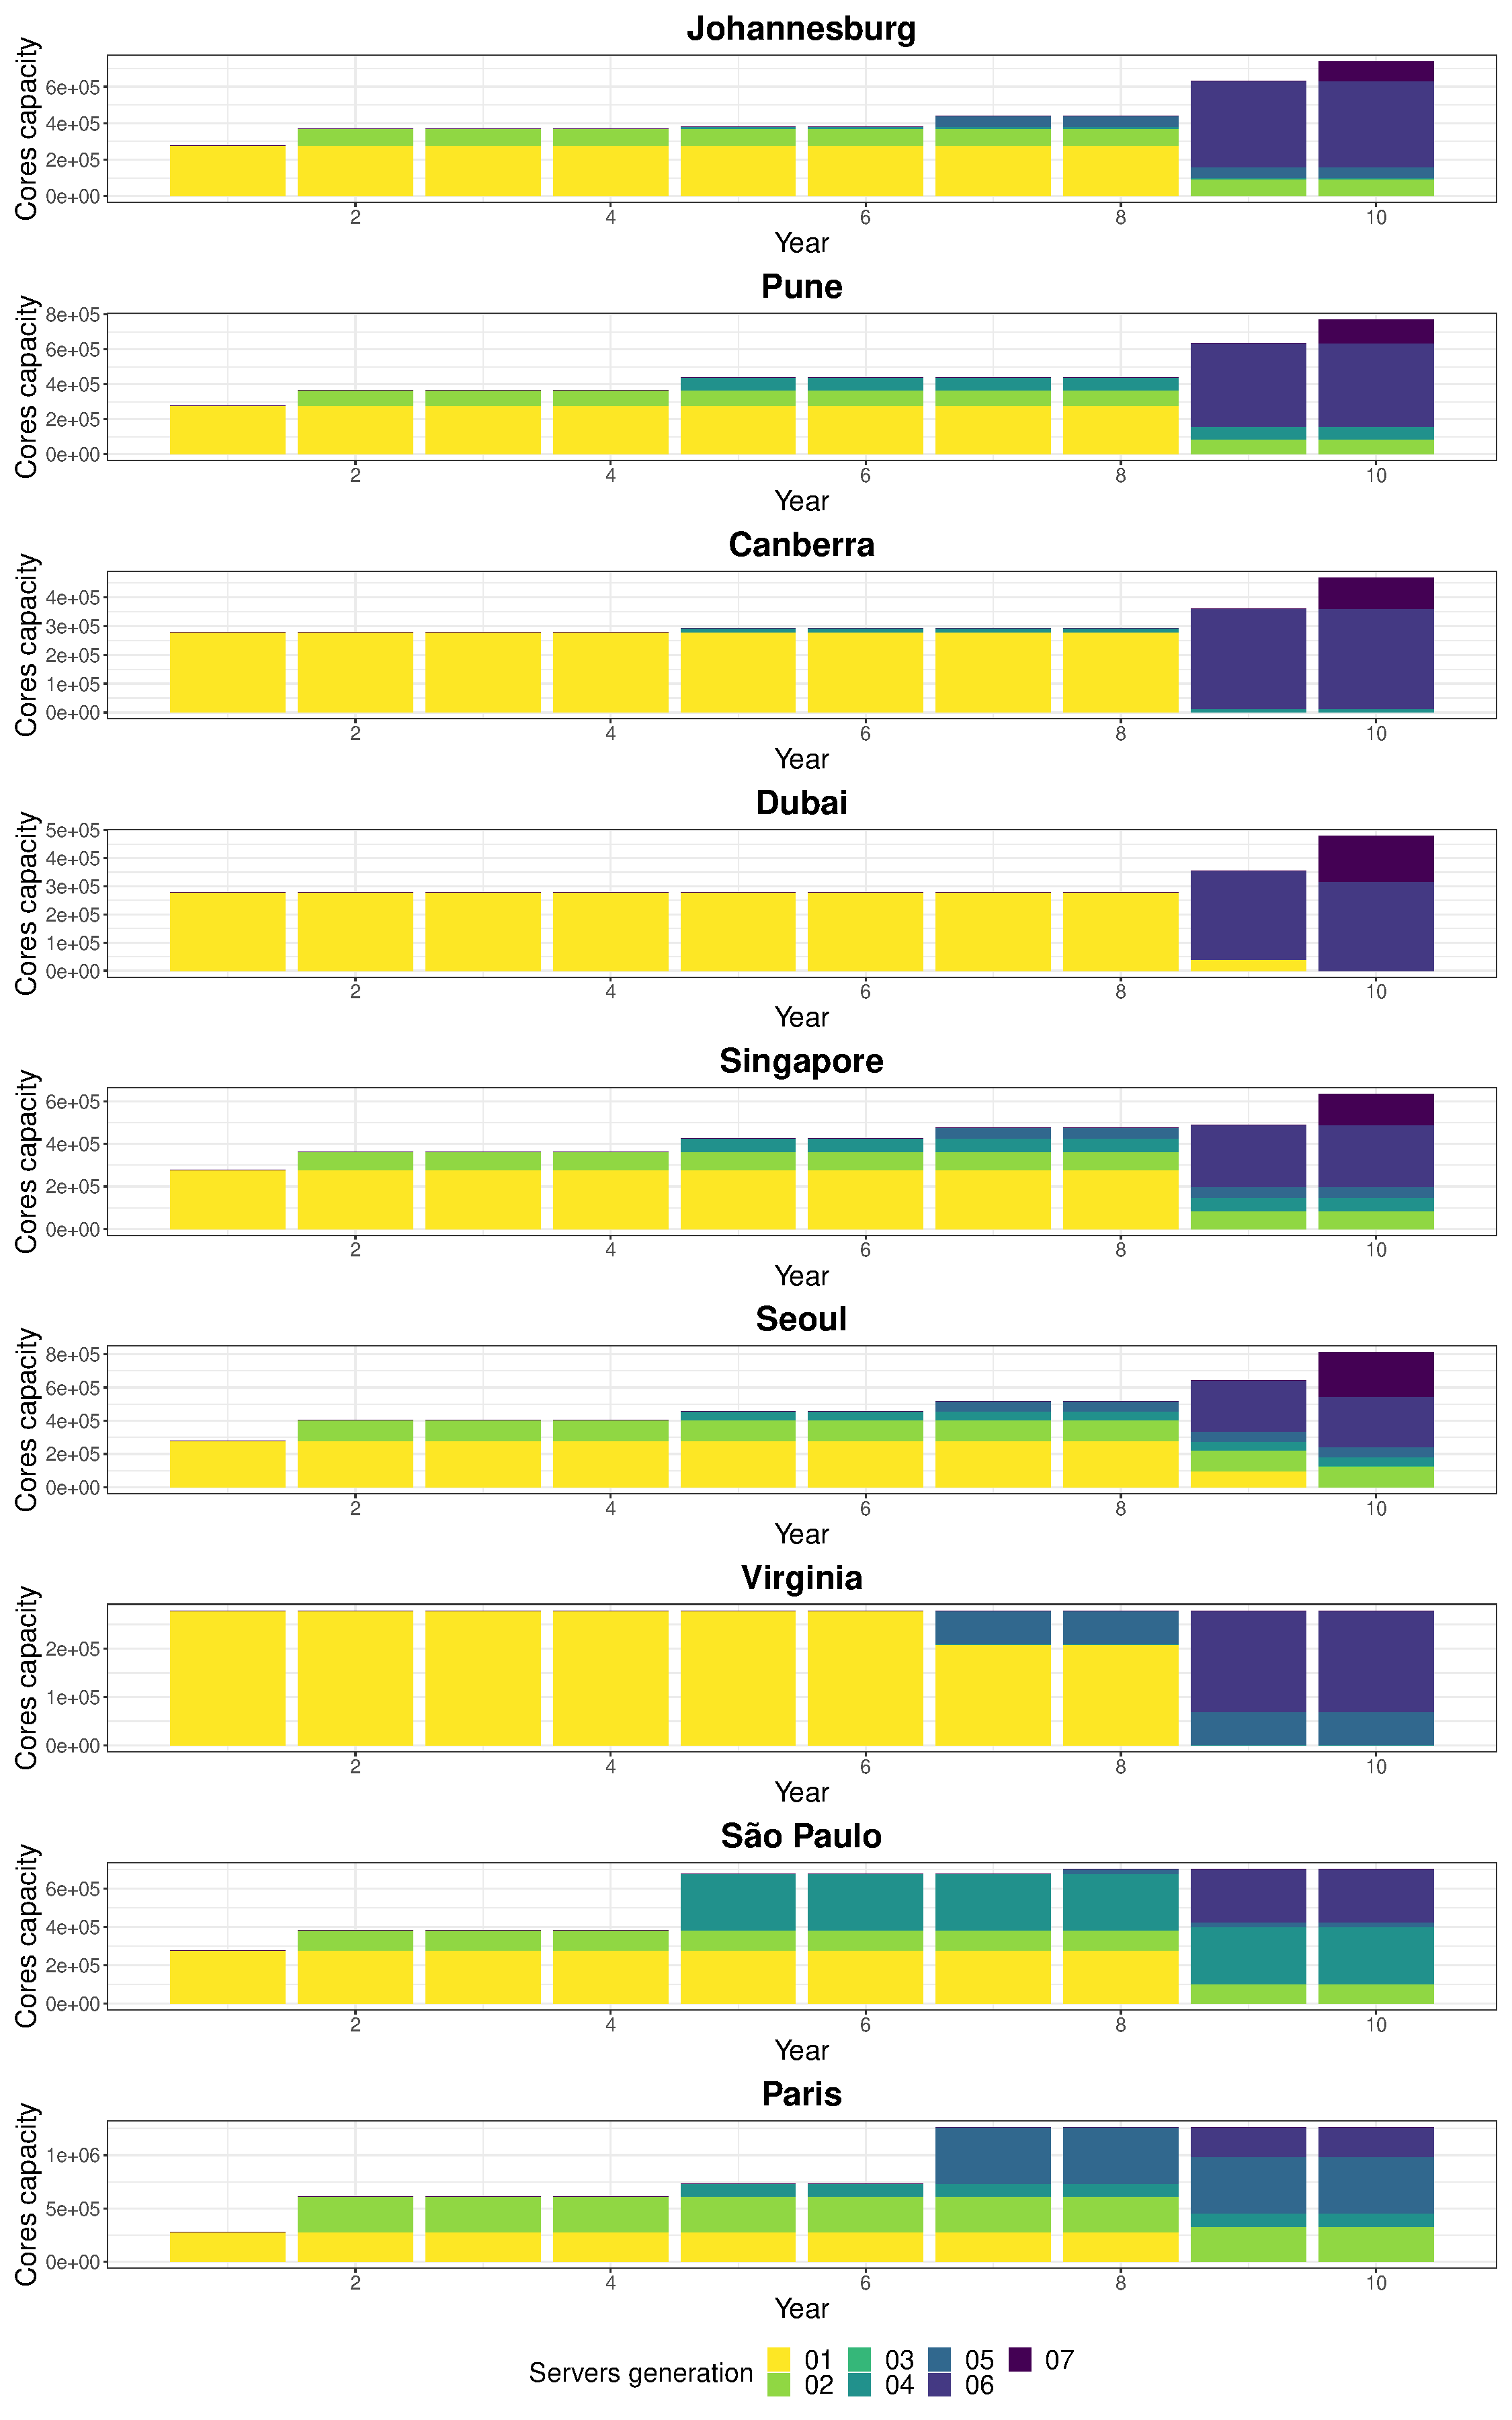
\includegraphics[width=\linewidth]{images/dc_evolution_optimal.pdf}
  \caption{Cloud federation evolution knowing all the information of the 10 years --- optimal solution.}
  \label{fig:dc_evolution_optimal}
\end{figure}

\begin{table}[!ht]
  
\caption{Total emissions for the different scenarios.}\label{tab:emissions_sizing} \centering

\begin{tabular}{|l|r|}
  \hline
  \textbf{Scenarios} & \textbf{Emissions ($t\,\ch{CO2}-eq$)}   \\
  \hline  
   Sizing with all the information of the 10 years  & 239620.06     \\  
  \hline
  Sizing with information of the current year       & 266035.35     \\
  \hline

\end{tabular}
\end{table}

%%% Add dcu, workload ratio e outras paradas ...
%%% co2 de servidores por ano ...


\section{Discussion}
\label{sec:long_term_discussion}

In this section, the reader will be presented to an analysis of the experiments and their results. The scope of the study is how to reduce the environmental impact that comes from the long term operation of a cloud federation --- in terms of \ch{CO2} emissions --- by adding locally installed renewable infrastructure: solar panels, wind turbines, and batteries (to deal with intermittency). One must not neglect that the renewable infrastructure also emmits carbon during its whole life time. We made the modifications in our modeling --- that initially only considered emissions from manufacturing --- and, as expected, there was a increase in the total emissions --- around 8\%. It is also possible to observe that the area of PVs were reduced on most of the locations --- Figure ~\ref{fig:pv_lca}, with the exception of Johannesburg. This could be explained by the fact that Johannesburg is the location that receives the most solar irradiation throughout the year, so it could compensate for the decrease of PV area in the other locations. Regarding the batteries, the reduction in Pune, Seoul and Singapore could be justified by the smaller PV area, as there will be less energy to store. On the other hand, we see an increase in the the battery capacity for the other locations. This could be justified by having a smaller PV area the renewable energy cannot be wasted. Finally, including the life cycle aspect makes our modeling more adequate to real life, and the emissions are still betterbetter than the scenario where only power from the local electricity grid is used in terms of carbon footprint --- 81\% in the scenario with PV and batteries.  

% talk abou tadding wind turbines
Regarding the wind turbines, we saw that including them in the renewable infrastructure has a significative positive impact on the carbon footprint of operating the cloud federation: a 34\% reduction in \ch{CO2} emissions in comparison to only using solar panels and batteries. Nevertheless, the number of necessary wind turbines to manufacture is quite high, and this is a problem considering the land area requirements of wind turbines. One study from NREL that evaluated the land area requirements at the United States and it reports that the relation between wind power production and required land area is 3.0 ± 1.7 MW/km² \cite{wtlanduse_2009}. Taking into account that in our experiments we considered wind turbines with a rated power of 1.5MW, this implies that for each square kilometer it is possible to install from one up to three wind turbines. This would not be possible for data centers located in urban centers that are highly populated. For example, in the case of Paris --- the one that had the lowest number of wind turbines --- we would need from 7 to 23 km², and in the case of Seoul --- the one with highest number of wind turbines --- it would require from 36 to 110 km².

% talk about sizing sensitivity

As said in Chapter~\ref{chap:ccgrid}, solar irradiation has a lower variance than wind speed and this reflects on the quality of the sizing process. We saw that in the comparison of the optimal scenario --- for the renewable infrasctructure that only considered PV panels and batteries, the sizing process that used simple estimation techniques (average and median values) had precise results, being up to 3\% worse than the optimal scenario (Table ~\ref{tab:co2_10y_pv_only}). For the scenario where we also included WT in the renewable infrastructure, we saw in Table ~\ref{tab:co2_10y_pv_only}) that it became less precise --- up to 12\% worse than the optimal. On the other hand, even in the worse case the reduction in total \ch{CO2} emissions by using the wind is significative: the worst scenario for PV + WT + Bat has a 17\% lower carbon footprint than the scneario with PV + Bat.

% TODO completar com cenarios q tem os valores la do ano ...
In what concerns the sensitivity of the model to the grid emissions input, we saw that the initial modeling that uses the average value  of the year is robust: using the hour by hour value reduces the total \ch{CO2} emissions  by less than 1\% --- as seen on Table X. This result presents a positive outcome, considering that not every location provide fine-grain value of the carbon intensity of its electricity grid.

% talk about flexibility in the scheduling
On the topic of exploring the flexibility in the scheduling of the workload to reduce carbon emissions, it is possible to extract the following information from the results. The first is that the reduction on the carbon footprint seems to have a limit ( around 4\%). This can be justified by the fact that there are no much difference in the climate conditions during the interval of one week, or that the DC which would reduce the carbon emissions is already at peak capacity and cannot receive more workload. The second interesting observation is that by delaying a small portion of the workload (for example 10\% to 20\%)  the reduction is already really close to the maximum possible reduction value. Finally, this approach can be used to reduce the impact of renewable sources' intermittency in the sizing process --- as we saw differences from 1\% to 12\% in comparison to the optimal scenario  on Section~\ref{sec:sensitivity} --- and in the context of cloud federations that emits from tens to hundreds of kilotons of \ch{CO2} eq, a reduction of 4\% is not negligible.

% Talk about price ...
Concerning the costs of reducing the environmental impact of the cloud operation --- one of the most important variables for the decision-makers --- we see in Table~\ref {tab:total_price} that the hybrid configuration is already cheaper than using power only from the electrical grid --- the solution that aimed to minimize the cost of the cloud operation for 1 year is around 40\% cheaper and emits 35\% less \ch{CO2} as seen in Table~\ref{tab:total_co2_scenarios_costs}. We also see that using a combination of solar panels and wind turbines allows to further reduce costs. On the other hand, the solution that result in the smaller environmental impact ( Minimum \ch{CO2} PV + WT + Bat + grid ) is the most expensive: it presents a reduction of 88\% in \ch{CO2} emissions than the grid only scenario but is 36.27\% more expensive. The scenario where the renewable infrastructure is only composed by PV panels is the best in terms of costs and environmental impact: it has a price close to the grid only scenario --- only 4\% more expensive --- and has a reduction of 81\% in \ch{CO2} emissions.

% Talk about new servers ...

When considering the long term operation of cloud data centers, the evolution of the technology hardware and increase in computational workload is of significant concern as well. Furthermore, these two variables increases the uncertainty of the problem: how power-efficient will be the CPUs or how much the workload will increase in the next decade ? The approach presented in this chapter, where the choice of manufacturing new servers is made year by year is more close to what could be adopted by the decision-makers of cloud federations, and it presented good results: in comparison to the optimal scenario --- unlikely to be achieved as it needs all the information of future climate conditions, hardware characteristics and workload of 10 years --- it is x\% worse. Furthermore, we see that the servers are being used way more than the expected life time of 4 years: on the optimal scenario, the first generation is used up to x years. This is interesting to motivate extending the life time of servers, as they are computationally powerfull and discarding them presents other environmental impact other than carbon emisisons. 


Finally, all the modifications in the modeling does not change its computational complexity, we still uses only linear variables, and it can be solved optimally in polynomial time.


\section{Summary}


\label{sec:long_term_conclusion}

\begin{itemize}
  \item Ongoing work:  
  \item Studying the sensibility of the model to intermittency    
    \begin{itemize}      
    \item Simple methods are efficient (avg. or median of irradiation)
    \end{itemize}

  \item Other strategies to reduce the \ch{CO2} emissions
    \begin{itemize}      
    \item Wind power: 6\% of reduction
    \item Delaying workload: up to 1.57\% of reduction      
    \end{itemize}
    
  \item When to add/replace servers

    \begin{itemize}
      
    \item Year by year solution 8\% worse than the optimal

      
    \end{itemize}
    
   
  \end{itemize}

  Future work:   Sizing for the long term :

  \begin{itemize}
    
  \item What could be learned from the optimal solution of adding/replacing servers ?

  \item Costs of the servers     

  \item Flexibility in the scheduling to reduce the number of
    servers manufactured

  \item Degradation of the renewable infrastructure over the years
    
  \end{itemize}

  
  All the extensions in the model are linear, so it does not extends the complexity of the modeling ...
